\documentclass[11pt,a4paper]{article}

\usepackage{fullpage}
\usepackage{hyperref}
\usepackage{graphicx}
\usepackage{amsmath}
\usepackage{tabu}
\usepackage{titlesec}
\usepackage{fancyhdr}
\pagestyle{fancy}
\fancyhf{}
\usepackage{todonotes}                %% notes from the authors

\setcounter{secnumdepth}{4}
\renewcommand{\headrulewidth}{0pt}
\renewcommand{\footrulewidth}{0pt}
\newcommand{\num}[1]{\texttt{#1}}

\fancypagestyle{firstpagefooter} {
	\lfoot{\tiny{Version: 25.09.2018}}
	\cfoot{}
	\rfoot{\thepage}
	
}

\lfoot{Name: Stefano Peverelli Legi: 19-980-396}
\rfoot{\thepage}

\begin{document}

\title{Advanced Systems Lab Report\\ \normalsize{Autumn Semester 2018}}
\author{Name: Stefano Peverelli\\Legi: 19-980-396}
\date{
	\vspace{4cm}
	\textbf{Grading} \\
	\vspace{0.5cm}
	\begin{tabular}{|c|c|}
		\hline  \textbf{Section} & \textbf{Points} \\
		\hline  1                &                 \\ 
		\hline  2                &                 \\ 
		\hline  3                &                 \\ 
		\hline  4                &                 \\ 
		\hline  5                &                 \\ 
		\hline  6                &                 \\ 
		\hline  7                &                 \\ 
		\hline \hline Total      &                 \\
		\hline 
	\end{tabular} 
}
\maketitle
\thispagestyle{firstpagefooter}

\newpage

\section{System Overview (75 pts)}

Following is a description of the class structure of the Middleware:

\begin{itemize}
    \item \texttt{MW} - responsible for accepting incoming socket connections, instantiating the \texttt{Writer} threads, and for enqueuing each request.
    \item \texttt{Request} - this class represent a request object, it contains the request's type and measures (presented below).
    \item \texttt{Worker} - each \texttt{Worker} establishes a socket connection with the memchached servers, dequeues a request, performs load balancing, and process the request (sends to servers, handle responses and collects some statistics.
    \item \texttt{Statistic} - container for all measured statistics.
    \item \texttt{Writer} - when shutting down the Middleware, it collects all the statistics from each \texttt{Worker}, aggregates them and save them to disk.
\end{itemize}

\begin{figure}[h]
    \centering
    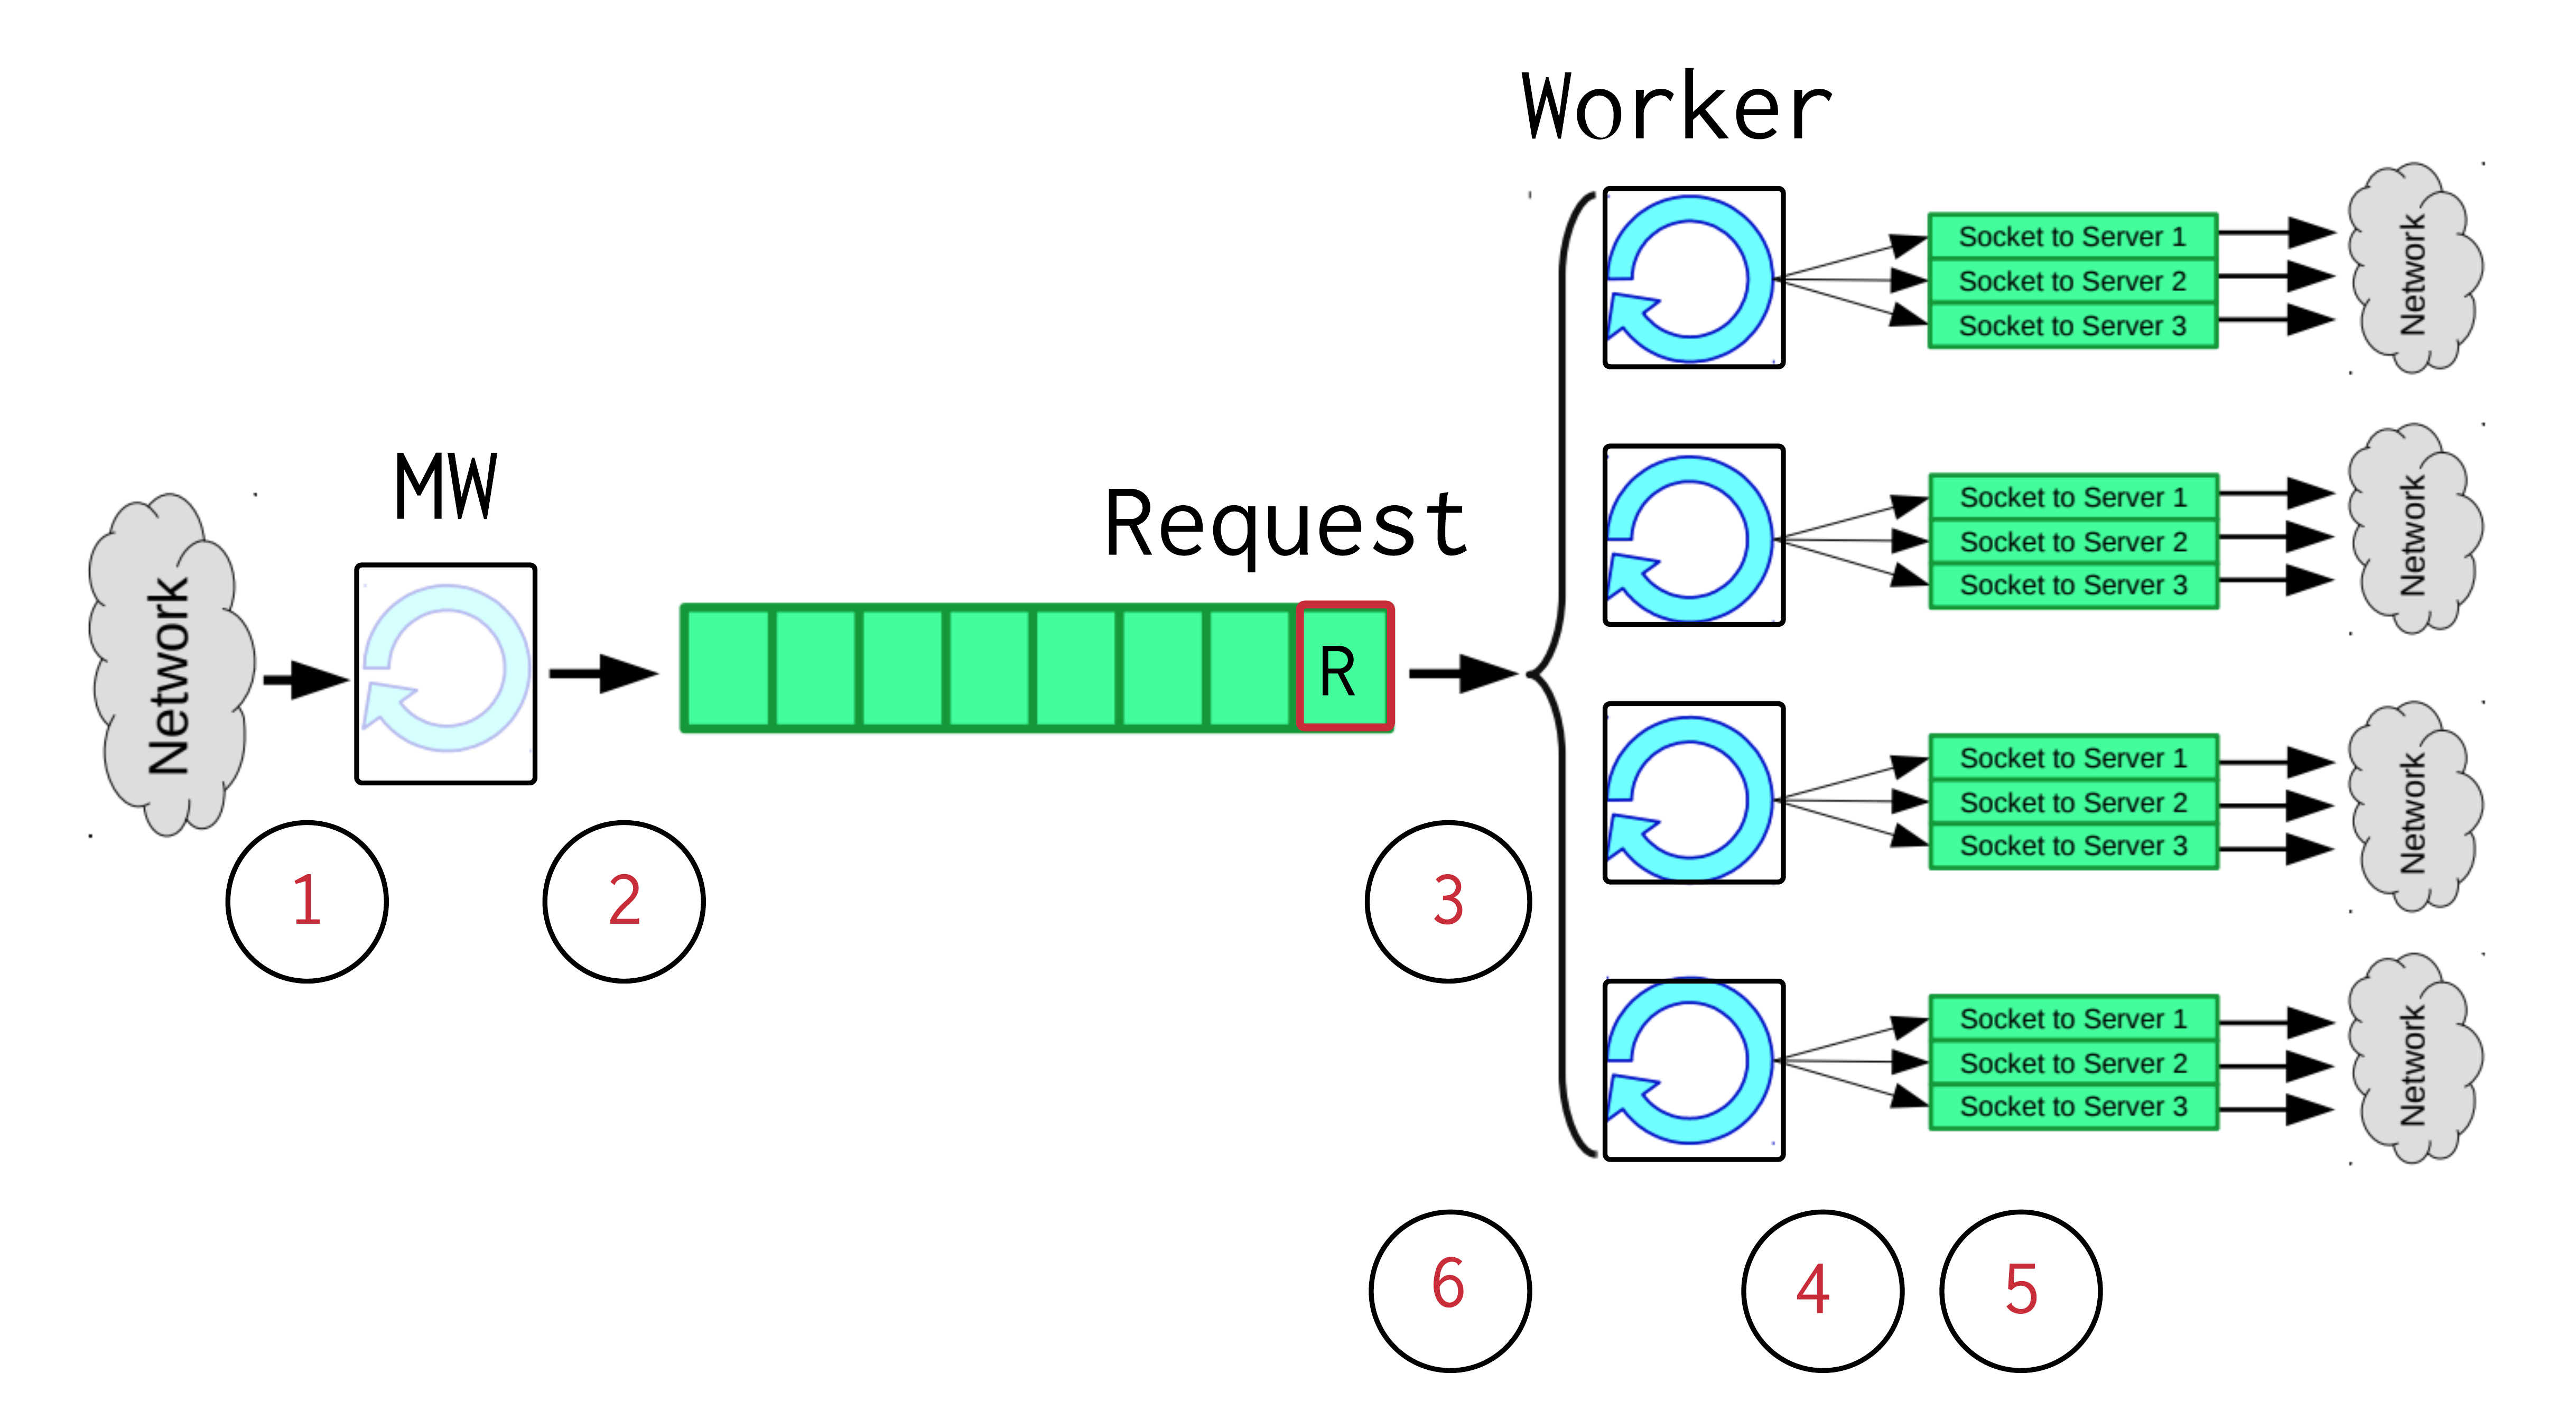
\includegraphics[width=0.8\textwidth]{figures/architecture.png}
    \label{fig:architecture}
    \caption{Middleware architecture.}
\end{figure}

The Middleware is instrumented at six points (shown in Fig.\ref{fig:architecture}):

\begin{enumerate}
    \item $R_{c}$ - Request created
    \item $R_{e}$ - Request enqueued
    \item $R_{d}$ - Request dequeued
    \item $R_{f}$ - Request forwarded to memcached instances.
    \item $R_{r}$ - Response received from memcached instances.
    \item $R_{a}$ - Request answered to memtier instance.
\end{enumerate}

\subsection{Load Balancing}

In order to guarantee that each server gets the same amount of jobs, each request's key gets hashed to a specific index that identify a memcached instance.\\This is done by method \texttt{getServerFromKey} in \texttt{Worker} class, and further tested in class \texttt{LoadBalancer} of package \texttt{test.java.asl}. Following is the result of a test with 1M random strings and 10 servers: \\\\
\texttt{
    Server 0 got 100047 jobs.\\
    Server 1 got 100172 jobs.\\
    Server 2 got 99590 jobs.\\
    Server 3 got 99714 jobs.\\
    Server 4 got 100506 jobs.\\
    Server 5 got 100081 jobs.\\
    Server 6 got 99962 jobs.\\
    Server 7 got 100221 jobs.\\
    Server 8 got 99809 jobs.\\
    Server 9 got 99898 jobs.\\}

This indeed shows that the distribution is uniform and that each memcached instance receives the same amount of requests as the others.\\\textbf{NOTE:} This is done only for \texttt{GET} and \textit{non-sharded} \texttt{MULTI-GET}s requests, as \texttt{SET}s need to be replicated, and \textit{sharded} \texttt{MULTI-GET}s are splitted across memcached instances. 

\subsection{The system}

There are two main components, the \texttt{MW} and the \texttt{Worker}s. They communicate between each other using a dynamic-sized queue where requests are passed in.

\subsection{The queue}

The queue is designed to grow as much as needed although in practice it can only grow to the number of clients memtier is using. A fixed-sized queue may have done the job as well, but having a dynamic-sized one has less impact on the memory usage.

\subsection{Non-blocking IO}

The Middleware communicate both with the clients and the memcached instances via the \texttt{java.NIO.SocketChannel}'s library. In \texttt{MW}'s constructor \texttt{Worker}'s are instantiated and started. Each \texttt{Worker}, connects to the memcached instances in a non-blocking fashion.

\subsection{Request Protocol}

Each request is assumed to be well-formed, and only the first character is checked in order to determine the request type. As a request may be sent into multiple chunks, it is essential to read it without losing any byte. Thisis done by saving the partial content of the \texttt{ByteBuffer} the \texttt{SocketChannel} has written to, into a \texttt{ByteArrayOutputStream}. A request is assumed to be completed when the last bytes are equals to\texttt{"\textbackslash{}r\textbackslash{}n"}. The same assumption is done for responses from the memcached instances, by checking \texttt{"STORED\textbackslash{}r\textbackslash{}n"} or \texttt{"END\textbackslash{}r\textbackslash{}n"}.

\subsection{Handling incoming connections}

The Middleware listens for incoming connections by memtier clients. This is achieved by using the \texttt{java.NIO} package that allows non-blocking IO operations on multiple channels. A \texttt{Selector} monitors channels for changes and signal them in a \texttt{SelectionKey} object, which contains a set of keys registered with the channel. \\Whenever a \texttt{SelectionKey}'s interest is set on \texttt{ACCEPT}, a \texttt{SocketChannel} connection can be established between the client issuing the request and the Middleware. After that, the interest of the \texttt{SelectionKey} is set to \texttt{READ}, waiting for data from the client.

\subsection{Handling incoming requests}

When the \texttt{SelectionKey}'s interest is set to \texttt{READ}, data is read from the \texttt{SocketChannel}. From this moment the Middleware starts recording the \texttt{responseTime} of the request (Point 1 in Fig.\ref{fig:architecture}). When the whole request has been read, it gets enqueued to a \texttt{BlockingQueue}, its \texttt{queueWaitingTime} is started (Point 2 in Fig.\ref{fig:architecture}), and the \texttt{SelectionKey}'s interest is set to \texttt{WRITE}.

\subsection{Forwarding requests}

When a new request is ready to be processed by a \texttt{Worker}, before sending it to the memcached instances, some operations take place (shown in Fig.\ref{fig:dequeue}):

\begin{itemize}
    \item The request's \texttt{queueWaitingTime} is stopped (Point 3 in Fig.\ref{fig:architecture}).
    \item The request gets copied into a \texttt{pendingRequest} object.
    \item Based on its type, a \texttt{multiRequest} object gets created.
\end{itemize}

Then, when the first entry of the \texttt{multiRequest} object gets sent, the \texttt{pendingRequest}'s \texttt{serviceTime} is started (Point 4 in Fig.\ref{fig:architecture}).

\begin{figure}[h]
    \centering
    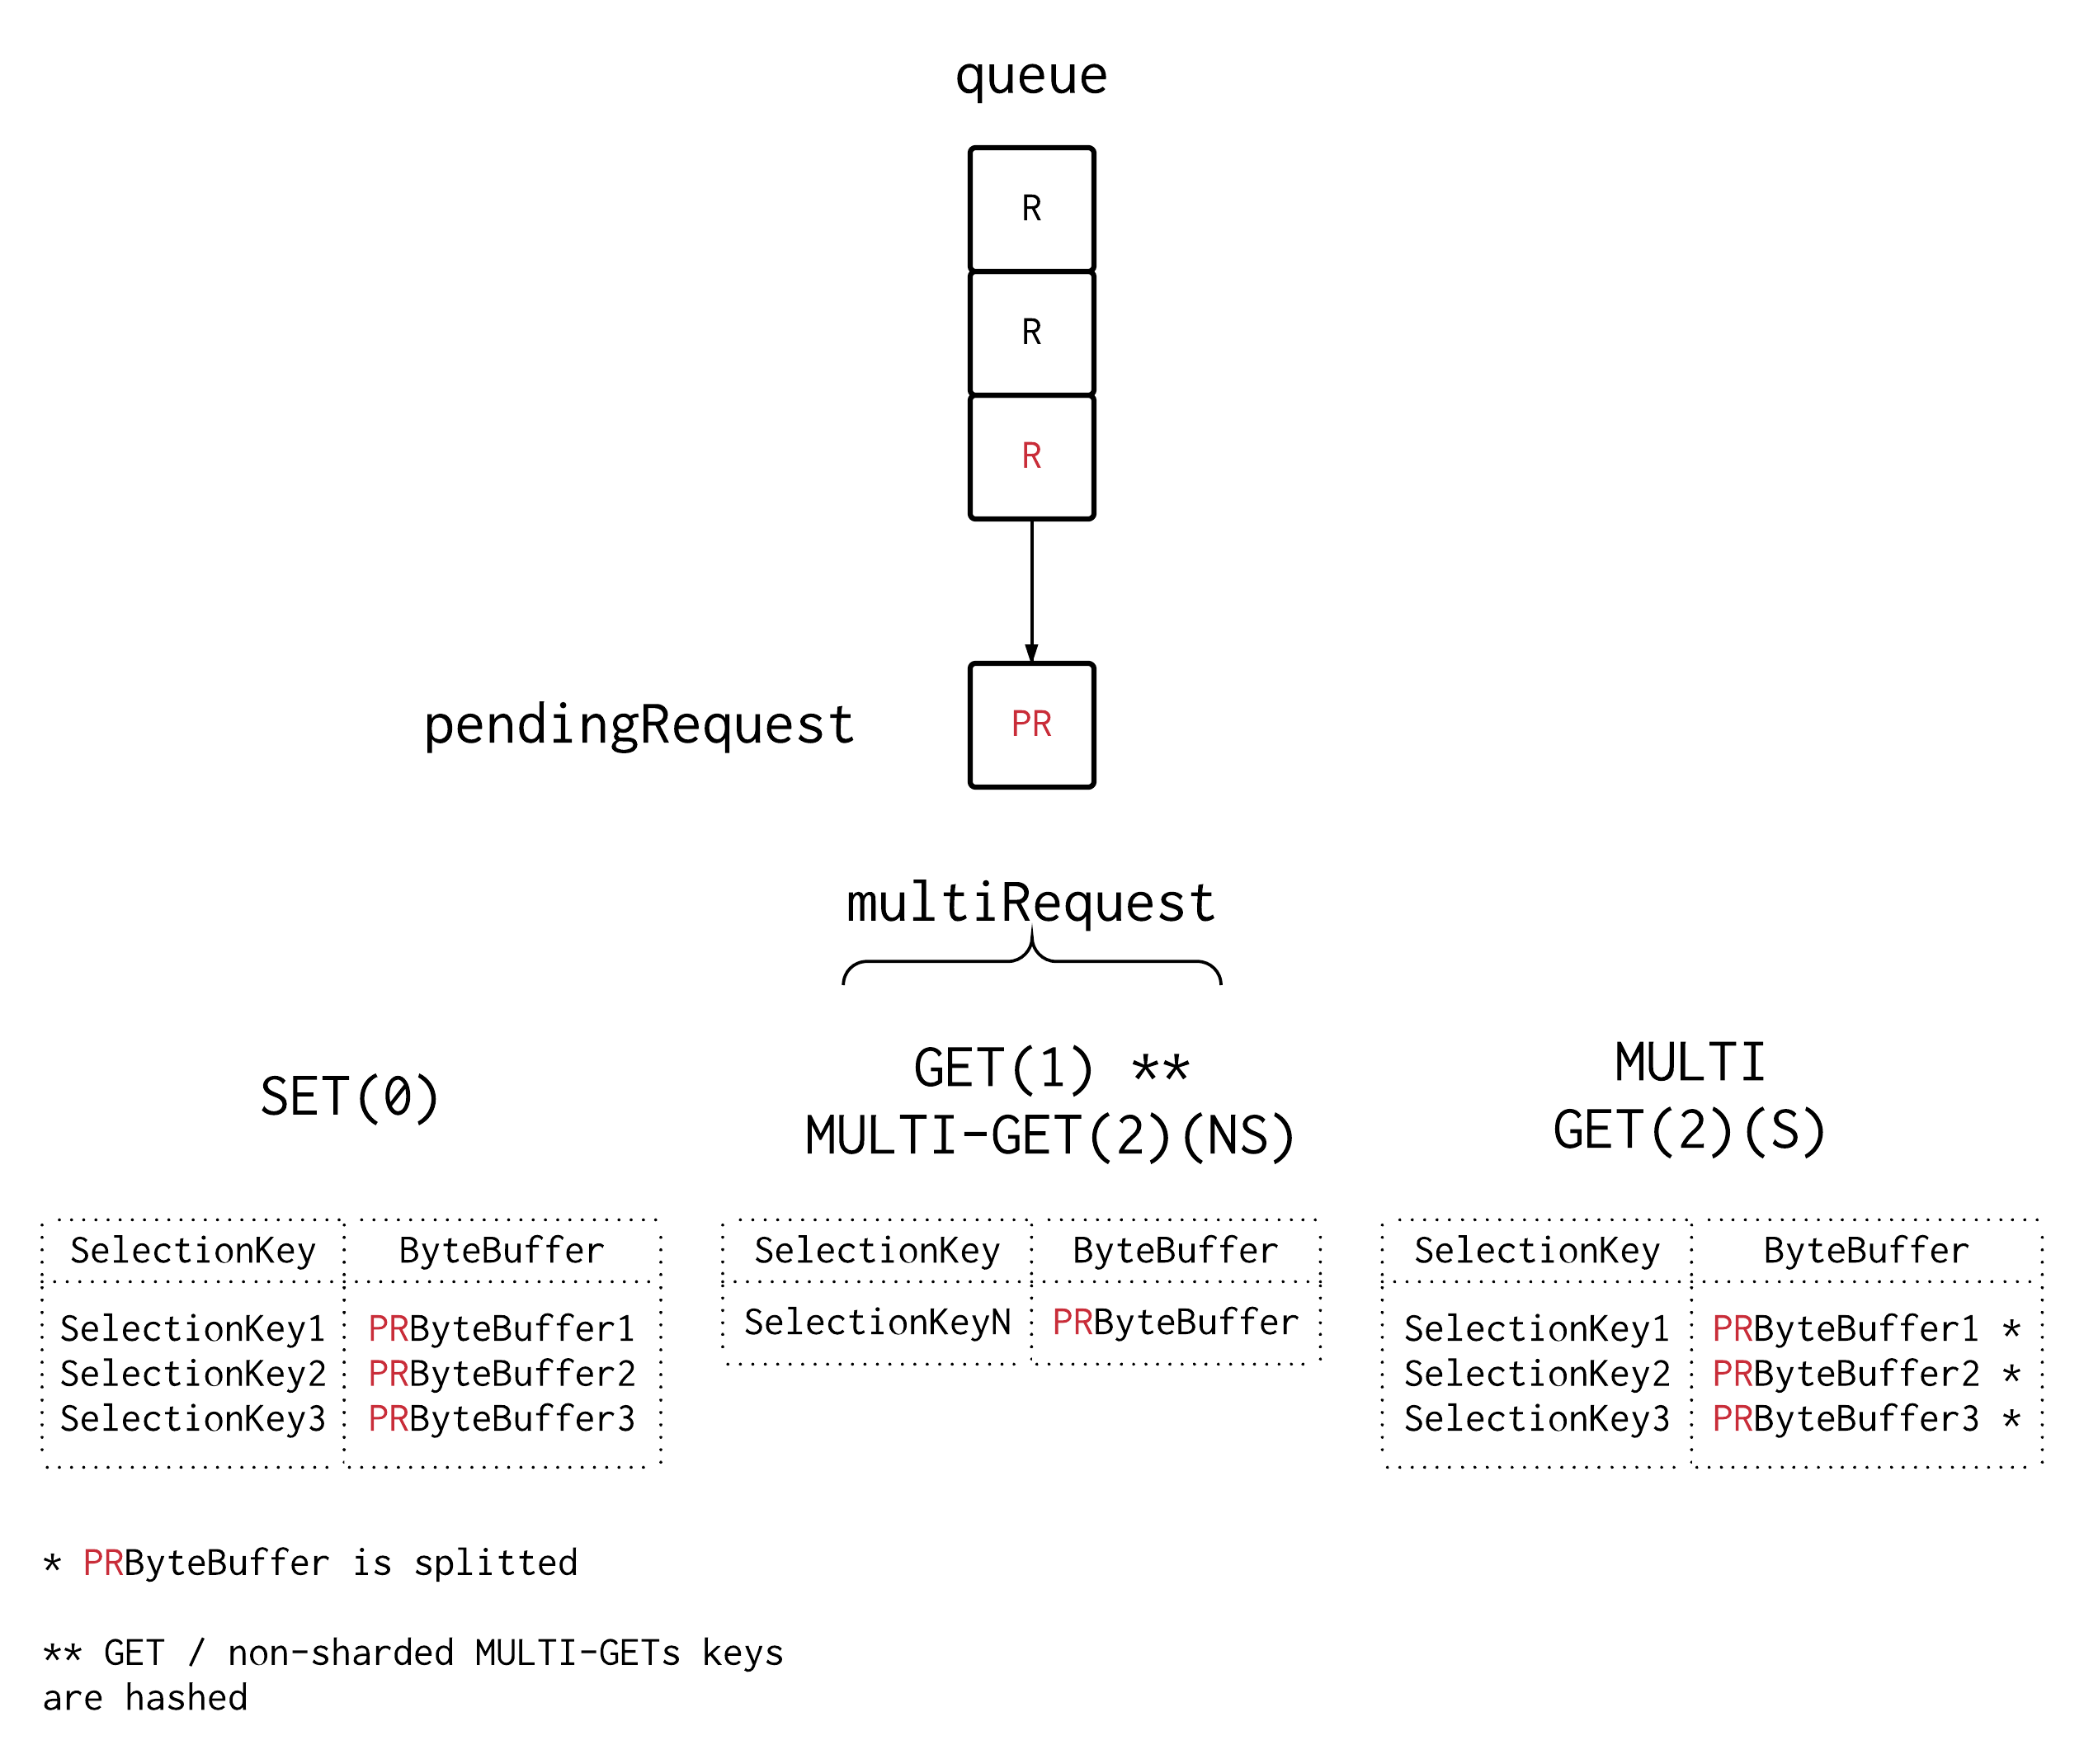
\includegraphics[width=0.9\textwidth]{figures/dequeue.png}
    \label{fig:dequeue}
    \caption{\texttt{loadRequest()} behavior.}
\end{figure}

\subsection{Handling responses}
\label{sec:responses}

When handling an incoming response each \texttt{Worker} does the following:

\begin{itemize}
    \item Checks if the response is completed
    \item Increments a counter of the number of responses received, and compares it with the size of the \texttt{multiRequest} object created for that \texttt{pendingRequest} (expected number of responses).
    \item Then, in case it has received the expected number of responses:
        \begin{itemize}
            \item Stops the \texttt{pendingRequest}'s \texttt{serviceTime} (Point 5 in Fig.\ref{fig:architecture}).
            \item Creates a \texttt{Statistic} object that wraps \texttt{pendingRequest} measures.
            \item Answers back to the client that issued the request.
            \item Stops the \texttt{pendingRequest}s \texttt{responseTime} (Point 6 in Fig.\ref{fig:architecture}).
        \end{itemize}
\end{itemize}        

\subsection{Statistics}
\label{sec:1.10}

As already pointed out in \ref{sec:responses}, each \texttt{Worker} collects the following statistics:

\begin{itemize}
    \item The current system's time (\texttt{ns}).
    \item The time the request spent in the queue (\texttt{ns}).
    \item The time elapsed between forwarding the first \texttt{multiRequest} and the last response (\texttt{ns}).
    \item The time elapsed between reading the request from the client and the last response (\texttt{ns}).
    \item The current queue size.
    \item The number of misses of the request.
    \item The number of keys in the request.
\end{itemize}

\textbf{NOTE:} All the time-related statistics are then converted in milliseconds (\texttt{ms}) when writing them to the logs.

\section{Baseline without Middleware (75 pts)}

In these experiments we study the performance characteristics of the memtier clients and memcached servers.

\subsection{One Server}
\label{sec:2.1}

In this, and in each of the following sections, the number of virtual clients is intended to be the total number of clients in the system, if otherwise, it is emphasized the phrase \textit{per thread}.
Bottleneck analysis, and throughput/response time comparsions are shown in each \textit{Explanation} section of each experiment, rather than in the Summary.
The focus on the latter is in presenting how the maximum throughput configurations are determined.

\subsubsection{Experiment Setting}

There are 3 machines that generate write-only and read-only workloads. Each machine runs a single memtier instance with 2 threads, and from a minimum of 1, to 64 virtual clients \textit{per thread} (see table below).
The number of virtual clients is the only (tunable) parameter in this setting; it is expected that by raising it, both throughput and response time should grow respectively. The reason behind it is that by raising the number of clients, the server  will spend less "idle/free time" between each successive request.
The clients machines are connected to a server machine running a single, one-threaded, memcached instance. Each experiment runs for 70 seconds (measures take into account both warm-up and cool-down phases, excluding 10 secs), and is repeated for 3 times under the same exact conditions.
By running this benchmark, we hope to find how much load can a single memcached instance sustain.

\begin{center}
	\scriptsize{
		\begin{tabular}{|l|c|}
			\hline Number of servers                & 1                        \\ 
			\hline Number of client machines        & 3                        \\ 
			\hline Instances of memtier per machine & 1                        \\ 
			\hline Threads per memtier instance     & 2                        \\
			\hline Virtual clients per thread       & [1, 4, 8, 16, 24, 32, 40, 48, 64]\\ 
			\hline Workload                         & Write-only and Read-only \\
			\hline Multi-Get behavior               & N/A                      \\
			\hline Multi-Get size                   & N/A                      \\
			\hline Number of middlewares            & N/A                      \\
			\hline Worker threads per middleware    & N/A                      \\
            \hline Repetitions                      & 3 (70 secs, effective 60 secs) \\ 
            \hline Log Files Path                   & \texttt{experiments/baseline\_no\_mw\_1\_server/} \\
            \hline Processed Files Path             & \texttt{experiments/baseline\_no\_mw\_1\_server/out/memtier\_data.csv}\\
            \hline
		\end{tabular}
	} 
\end{center}

\subsubsection{Explanation}

The following plot shows how throughput and reponse time behave when increasing the number of virtual clients.
The number of virtual clients on the \texttt{x-axis} of each plot represents the total number of clients in the system, e.g. the first tick at \texttt{VC=6} is the result of \texttt{1} virtual client per thread multiplied by the number of threads (\texttt{2}), instances(\texttt{1}), and client machines(\texttt{3}).
For each quantity we plot the average measured value of the 3 repetitions, and the standard deviation from the mean as a confidence measure.
Additionally as a sanity check, we plot the \textit{Interactive Law} as a dotted line in the troughput plots.
In this case it is computed as the invers of the measured response time multiplied by the total number of virtual clients.
The throughput shown below is the sum of the throughputs of each memtier instance of each client, while the response time is the average response time of each client's machine. 

\subsubsection*{Read-Only}

Consider the throughput below: we can see pretty clearly that, for the whole virtual clients range, apart from \texttt{VCs=6}, (in which the memcached server is still \textbf{under-saturated}), it essentially remains constant at $\approx 3000$ops/s. Suprisingly, increasing the number of virtual clients doesn't affect the throughput at all; the server is indeed saturated after 6 virtual clients. Although we have extended the range of virtual clients per thread to 64, we still cannot observe over-saturation of the server.\\
The same exact behavior can be double checked by looking at the response time plot. It grows almost linearly, confirming the fact that the server is saturated.\\ As for now, (without additional information both on the arrival rate of requests and the service rate at which they get processed), we cannot determine the bottleneck of the sytem. Either outbound load is limited by the client's bandwidth, or the server's peak performance in reading is 3k ops/s. In Section~\ref{sec:2.2} we investigate how much workload a client machine can generate, that is the missing piece of the puzzle to conclude the bottleneck analysis.

\begin{figure}[!h]
  \centering
  \caption{Plots for baseline with one server (read-only)}
  \label{fig:baseline_no_mw_1_server_ro}
  \makebox[\textwidth]{
    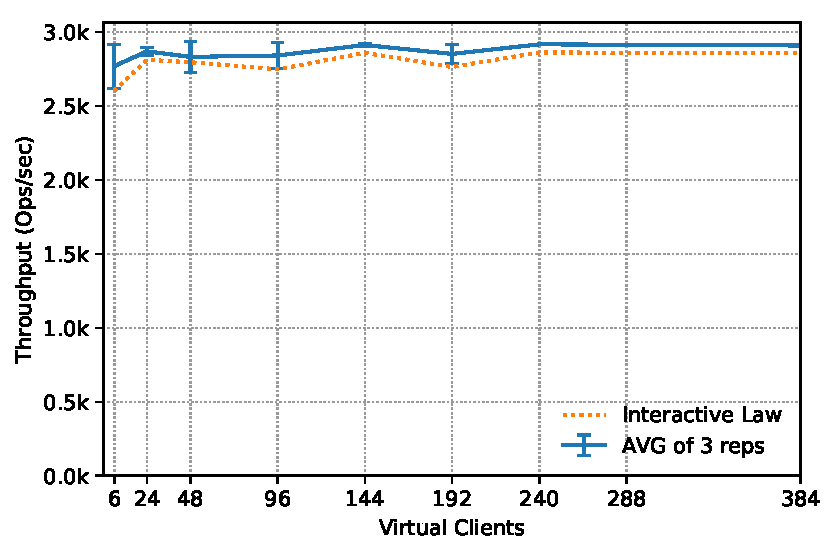
\includegraphics[width=0.6\textwidth]{figures/baseline_no_mw_1_server/tp_memtier_read_only.pdf}
    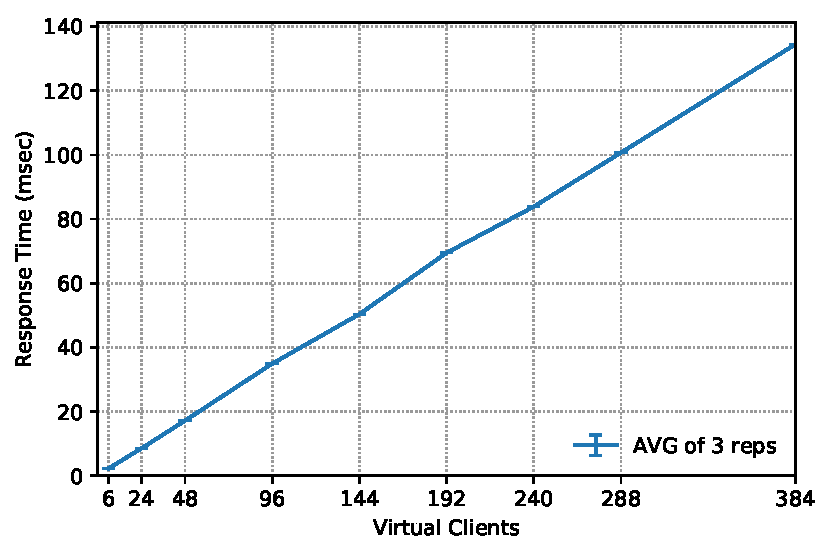
\includegraphics[width=0.6\textwidth]{figures/baseline_no_mw_1_server/rt_memtier_read_only.pdf}
  }
\end{figure}

\subsubsection*{Write-Only}

When testing for write-only workloads we observe a completely different behavior with respect to what seen above. Here the throughput follow our initial assumption and grows as the number of virtual clients increases. We can see that at \texttt{VCs=240} we reach saturation. We can explain the fact that we reach saturation at a much higher number of VCs compared to the read-only workload, simply because the service rate at which the server process write-only requests, is higher than when reading. This is investigated and further confirmed when measuring service time for different workloads inside the middleware in Section ~\ref{sec:3.1}.
With no surprise, the response time plot reflects the measured throughput: we have an initial under-saturated phase until \texttt{VCs=240}, for which the rate $\dfrac{r_t}{\texttt{VC}}$ monotonically decreases.
After that point, the rate stays almost constant, suggesting a flattening:\\\\
$\dfrac{2.5}{24}= \approx 0.1$\\\\
$\dfrac{4}{48}= \approx 0.08$\\\\
$\dfrac{6}{96}= \approx 0.06$\\\\
$\dfrac{12}{192}= \approx 0.06$\\\\
$\dfrac{14}{240}= \approx 0.058$\\\\
$\dfrac{22}{384}= \approx 0.057$\\\\
In addition, by looking at the interactive law, we can observe that it follows the throughput line precisely, concluding the analysis for the experiment.

\begin{figure}[!h]
  \centering
  \caption{Plots for baseline with one server (write-only)}
  \label{fig:baseline_no_mw_1_server_wo}
  \makebox[\textwidth]{
    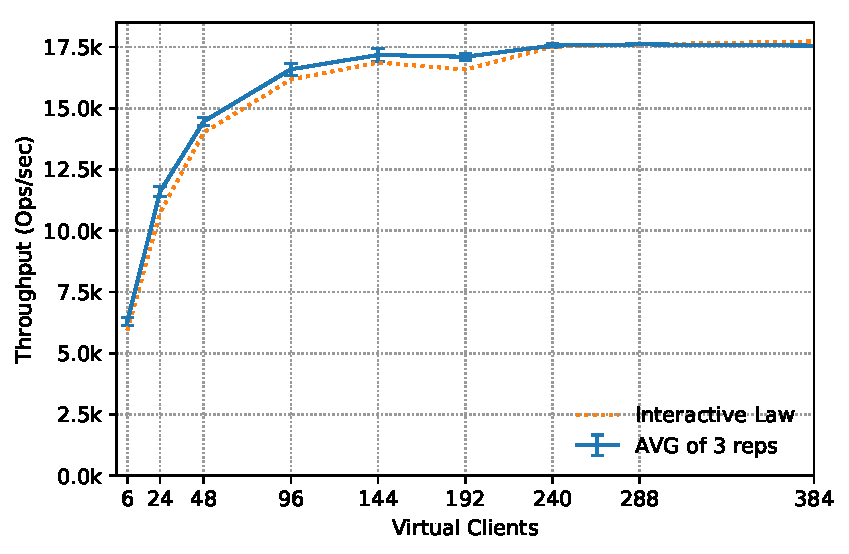
\includegraphics[width=0.6\textwidth]{figures/baseline_no_mw_1_server/tp_memtier_write_only.pdf}
    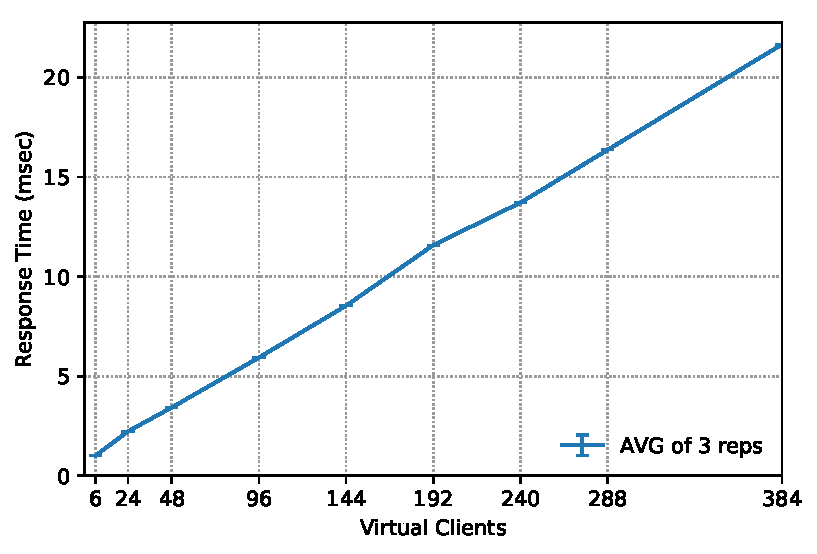
\includegraphics[width=0.58\textwidth]{figures/baseline_no_mw_1_server/rt_memtier_write_only.pdf}
  }
\end{figure}

\subsection{Two Servers}
\label{sec:2.2}

\subsubsection{Experiment Setting}

There is a single client machine that generates write-only and read-only workloads. The machine runs two different memtier instances with 1 thread, and from a minimum of 1, to 32 virtual clients (see table below).
The number of virtual clients is again, the only (tunable) parameter in this setting; it is expected that by raising it, both throughput and response time should grow accordingly. We connect each client's instance to 2 different server machines running a single, one-threaded, memcached instance. The same exact conditions on the number of repetions, duration and measurement stated before still hold. By running this benchmark, we hope to find how much load can a single memtier client produce before saturation.

\begin{center}
	\scriptsize{
		\begin{tabular}{|l|c|}
			\hline Number of servers                & 2                        \\ 
			\hline Number of client machines        & 1                        \\ 
			\hline Instances of memtier per machine & 2                        \\ 
			\hline Threads per memtier instance     & 1                        \\
            \hline Virtual clients per thread       & [1, 4, 8, 16, 24, 32]    \\ 
			\hline Workload                         & Write-only and Read-only \\
			\hline Multi-Get behavior               & N/A                      \\
			\hline Multi-Get size                   & N/A                      \\
			\hline Number of middlewares            & N/A                      \\
			\hline Worker threads per middleware    & N/A                      \\
            \hline Repetitions                      & 3 (70 secs, effective 60 secs) \\ 
            \hline Log Files Path                   & \texttt{experiments/baseline\_no\_mw\_2\_server/} \\
            \hline Processed Files Path             & \texttt{experiments/baseline\_no\_mw\_2\_server/out/memtier\_data.csv}\\
			\hline 
		\end{tabular}
	} 
\end{center}

\subsubsection{Explanation}

Once again we plot both throughput and response time as a function of the total number of clients. It is interesting to note how these quantities are measured. The response time is the mean response time of each memtier instance, for each client machine, for each repetition. The throughput is the sum of the throughputs measured in each instance, summed over the number of client machines, and averaged between each repetition. The error measure introduced is again the standard deviation from the mean value in all repetitions.

\subsubsection*{Read-Only}

The throughput presents an interesting behavior: as before, we observe that it flattens early on, at \texttt{VCs=8}, reaching saturation at $\approx$ 6k $ops/s$. From that point on, the system seems to begin to over-saturate, as the throughput slightly decrases.\\
In Section \ref{sec:2.1} we have 3 clients connected to one server, reaching peak performance at $\approx$ 3k $ops/s$, this suggests that now that we have a single client that can read 6k $ops/s$ from two servers, that the bottleneck when reading is effectively the service rate at which a single memcached instance process incoming requests. The response time, after a sub-linear growth between the first and second virtual clients grows linearly, confirming saturation.

\begin{figure}[!h]
  \centering
  \caption{Plots for baseline with two servers (read-only)}
  \label{fig:baseline_no_mw_2_server_ro}
  \makebox[\textwidth]{
    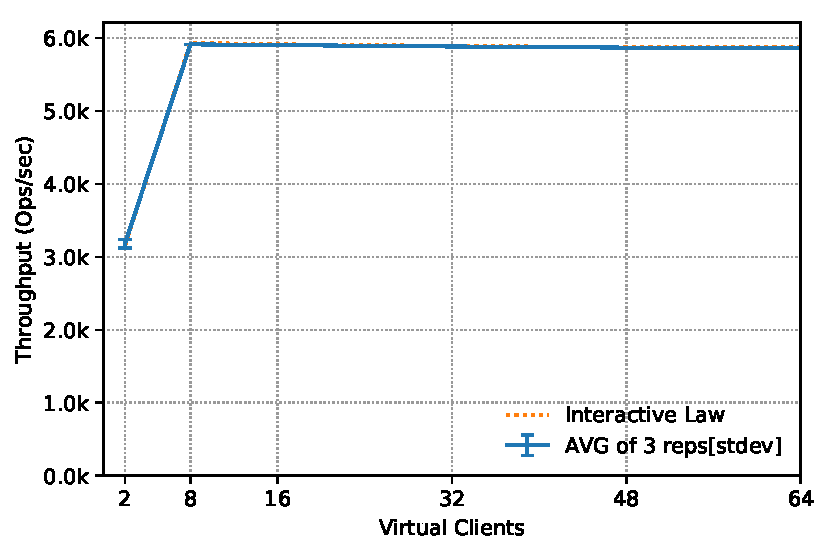
\includegraphics[width=0.6\textwidth]{figures/baseline_no_mw_2_server/tp_memtier_read_only.pdf}
    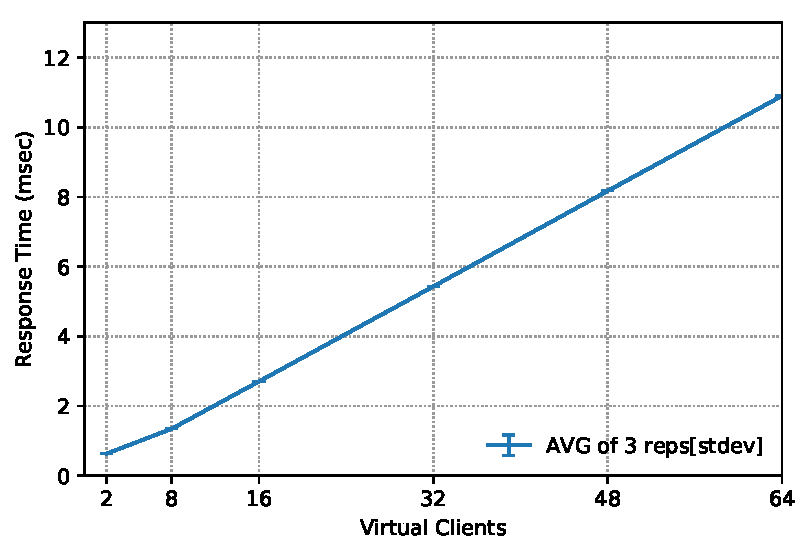
\includegraphics[width=0.6\textwidth]{figures/baseline_no_mw_2_server/rt_memtier_read_only.pdf}
  }
\end{figure}

\subsubsection*{Write-Only}

The throughput is almost identical to the read-only workload. Again a pretty fast flattening at $\num{VCs=8}$. 
Let's compare it with the one in Section \ref{sec:2.1}: there, we have 3 clients writing to a single server, reaching an $\approx$ 18k $ops/s$ peak performance), meaning an approximate throughput per client of 6k $ops/s$.
Now by doubling the number of servers, a single client still produces 6k $ops/s$. 
Thus, we can conclude that the bottleneck is the maximum arrival rate of incoming write-only request from a single client machine, limited at 6k $ops/s$. 

\newpage

\begin{figure}[!h]
  \centering
  \caption{Plots for baseline with two servers (write-only)}
  \label{fig:baseline_no_mw_2_server_wo}
  \makebox[\textwidth]{
    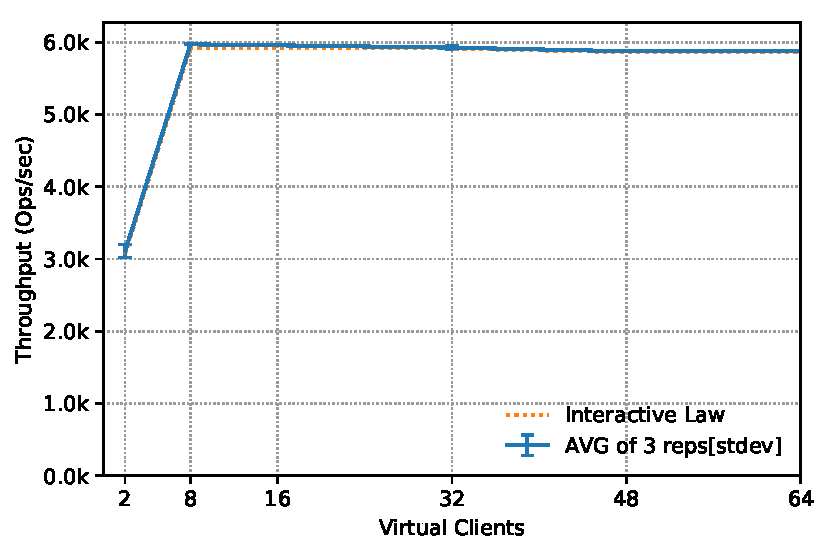
\includegraphics[width=0.6\textwidth]{figures/baseline_no_mw_2_server/tp_memtier_write_only.pdf}
    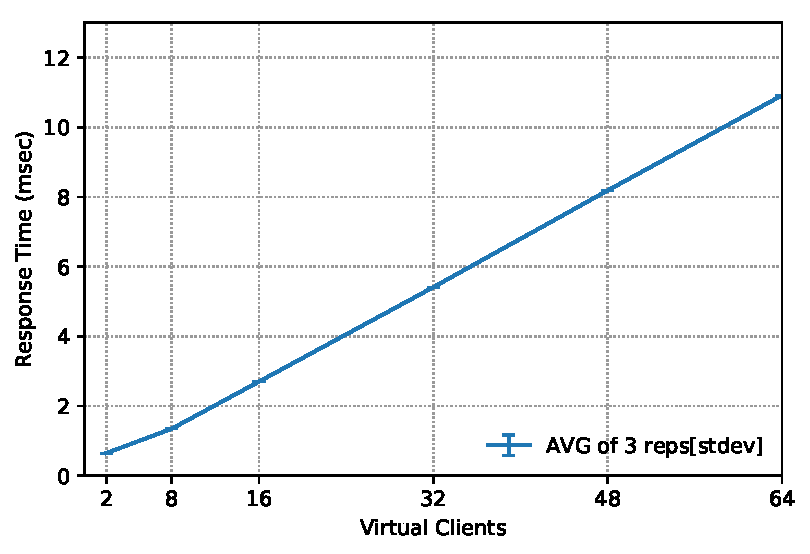
\includegraphics[width=0.6\textwidth]{figures/baseline_no_mw_2_server/rt_memtier_write_only.pdf}
  }
\end{figure}

\subsection{Summary}

Following, the maximum throughput of each experiment for both write-only and read-only workload is shown.
In order to determine what is the maximum throughput configuration, we additionally plot the rate of change of the response time over the generated load and pick the configuration from which the rate reaches an horizontal asyntote.
Before that point the response time can grow sub-linearly, even oscillating (in the read-only case). So, we choose the first stable virtual client which rate stays almost flat for the entire range of virtual clients to represent the maximum throughput configuration in our system.

\begin{figure}[!h]
  \centering
  \caption{Plots for baseline with one server (Rate of change of response time over load, left: read-only, right: write-only)}
  \label{fig:baseline_no_mw_1_server_maxtp}
  \makebox[\textwidth]{
    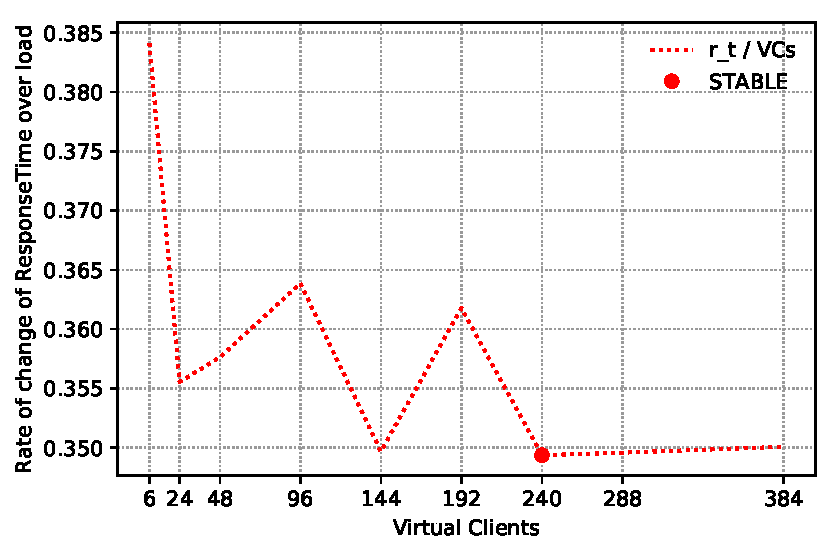
\includegraphics[width=0.6\textwidth]{figures/baseline_no_mw_1_server/maxtp_memtier_read_only.pdf}
    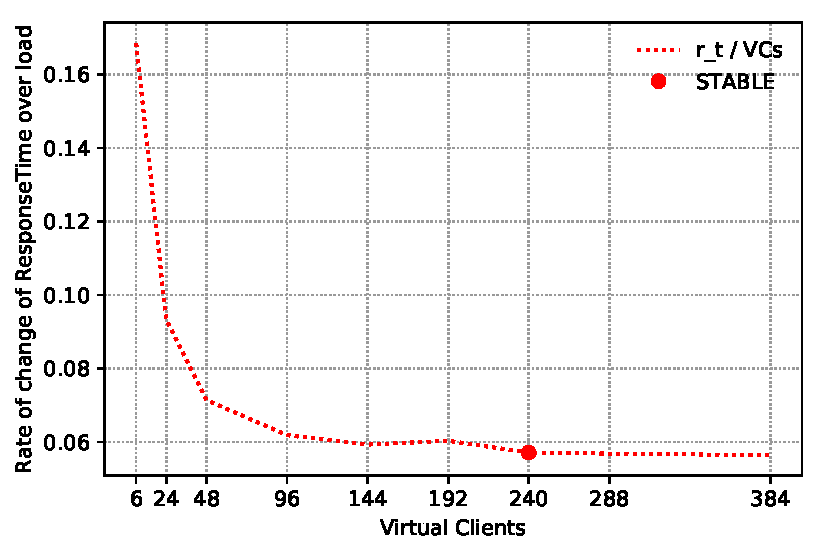
\includegraphics[width=0.6\textwidth]{figures/baseline_no_mw_1_server/maxtp_memtier_write_only.pdf}
  }
\end{figure}

\begin{figure}[!h]
  \centering
  \caption{Plots for baseline with two servers (Rate of change of response time over load, left: read-only, right: write-only)}
  \label{fig:baseline_no_mw_2_server_maxtp}
  \makebox[\textwidth]{
    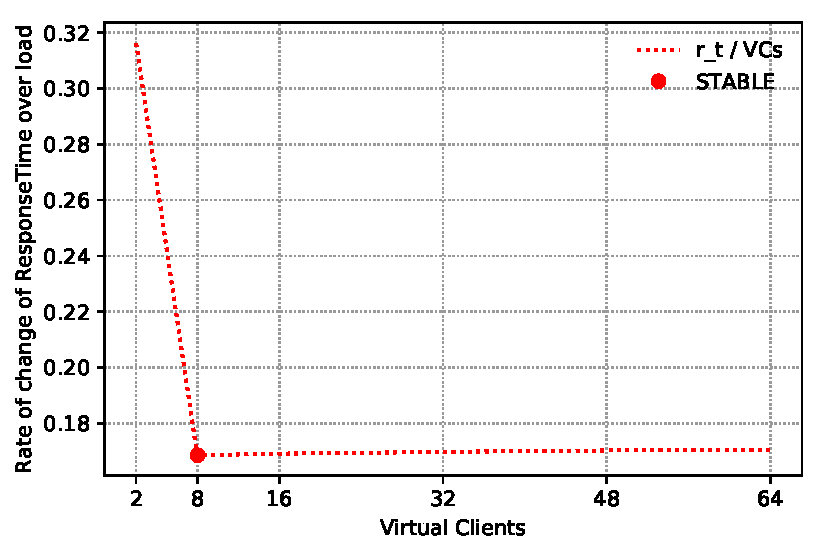
\includegraphics[width=0.6\textwidth]{figures/baseline_no_mw_2_server/maxtp_memtier_read_only.pdf}
    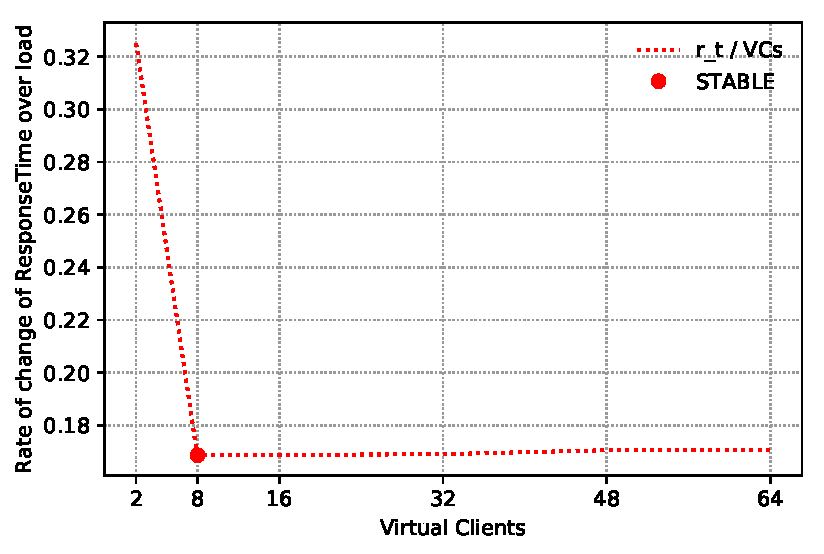
\includegraphics[width=0.6\textwidth]{figures/baseline_no_mw_2_server/maxtp_memtier_write_only.pdf}
  }
\end{figure}

\begin{center}
	{Maximum throughput of different VMs.}
	\begin{tabular}{|l|p{2cm}|p{2cm}|p{4cm}|}
		\hline                        & Read-only workload & Write-only workload & Configuration gives max. throughput  \\ 
        \hline One memcached server   & 2.88k ops/s        & 17.5k ops/s         & 40 VCs per thread (240 total clients)\\ 
        \hline One load generating VM & 5.87k ops/s        & 5.98k ops/s         & 4 VCs per thread (8 total clients)   \\  
		\hline 
	\end{tabular}
\end{center}


\section{Baseline with Middleware (90 pts)}
\label{sec:3.1}

In this set of experiments we test the performance of the Middleware/s. 
We measure and display the results both at the client, and inside the middleware, and compare them.
Additionally, in order to gain a better insight on the internal performance breakdown of the middleware, and run analysis on the components, we present the statistics introduced in Section \ref{sec:1.10}.

\subsection{One Middleware}

\subsubsection{Experiment Setting}

There are 3 clients machine generating both write-only and read-only workload. Each client machine runs a single memtier instance with 1 thread, and from a minimum of 1, to 64 virtual clients (see table below).
Each client machine is connected to the the middleware, which is connected to a single, one-threaded, memcached machine.
Essentially we are tuning the load the clients produce, and the service rate at which the middleware dispatches request between client and server machines. 

\begin{center}
	\scriptsize{
		\begin{tabular}{|l|c|}
			\hline Number of servers                & 1                        \\ 
			\hline Number of client machines        & 3                        \\ 
			\hline Instances of memtier per machine & 1                        \\ 
			\hline Threads per memtier instance     & 2                        \\
            \hline Virtual clients per thread       & [1, 4, 8, 16, 24, 32, 64]\\ 
			\hline Workload                         & Write-only and Read-only \\
			\hline Multi-Get behavior               & N/A                      \\
			\hline Multi-Get size                   & N/A                      \\
			\hline Number of middlewares            & 1                        \\
			\hline Worker threads per middleware    & [8, 16, 32, 64]                  \\
            \hline Repetitions                      & 3 (70 secs, effective 60 secs) \\ 
            \hline Log Files Path                   & \texttt{experiments/baseline\_mw\_1\_mw/logs} \\
            \hline Processed Files Path             & \texttt{experiments/baseline\_mw\_1\_mw/out/memtier\_data.csv}\\
            \hline
		\end{tabular}
	} 
\end{center}

\subsubsection{Explanation}

We plot throughput and response time as measured at the client and inside the middleware, for an increasing number of both virtual clients and  worker threads.\\
The measurements conducted in the middleware are grouped in five-seconds windows for a total of 14 per experiment ($ 70.0 / 5.0 = 14$). Everytime a request has been processed, and a response has been sent back to the client machines, the measurements for the specific request, and a snapshot of the system components, gets saved and later, processed and logged.\\
Measurements taken inside the middleware, do not include the latency between the client machines and the middleware, so there's a gap between the two, that remains constant and negligible ($\approx 2 ms$).

\subsubsection*{Read-Only}

As in Section \ref{sec:2.1}, the throughput plot shows a flattening at $\approx$ 3k $op/s$ starting from \texttt{VCs=24}.  The presence of the middleware doesn't seem to affect the performance at all, moreover we cannot spot any differences when changing the number of worker threads inside the middleware. The unique possible explanation, (as we can exclude the fact that the client machines are the bottleneck, from what we have concluded in \ref{sec:2.3}), is again. the fact that a single memcached machine cannot process more than $\approx$ 3k $ops/s$ incoming read-only requests. 

\begin{figure}[!h]
  \centering
  \caption{Plots for baseline with one Middleware (read-only CLIENT)}
  \label{fig:baseline_mw_1_mw_mt_ro}
  \makebox[\textwidth]{
    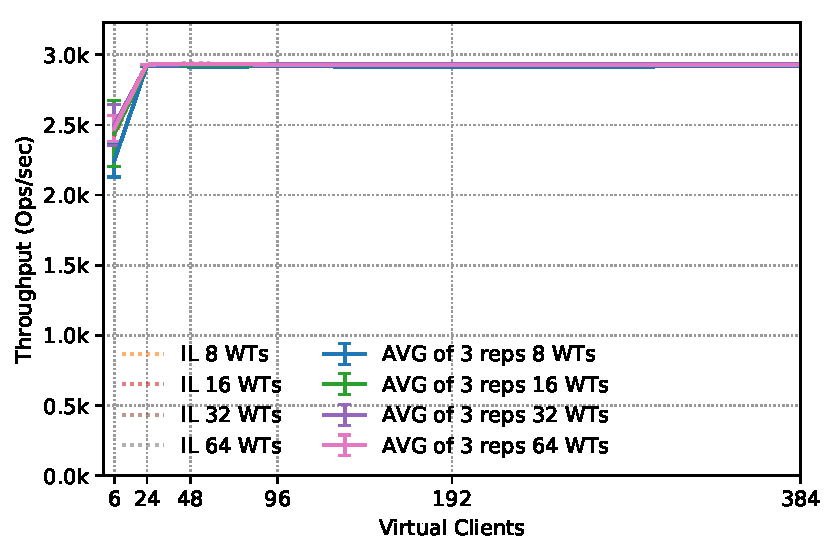
\includegraphics[width=0.6\textwidth]{figures/baseline_mw_1_mw/tp_memtier_read_only.pdf}
    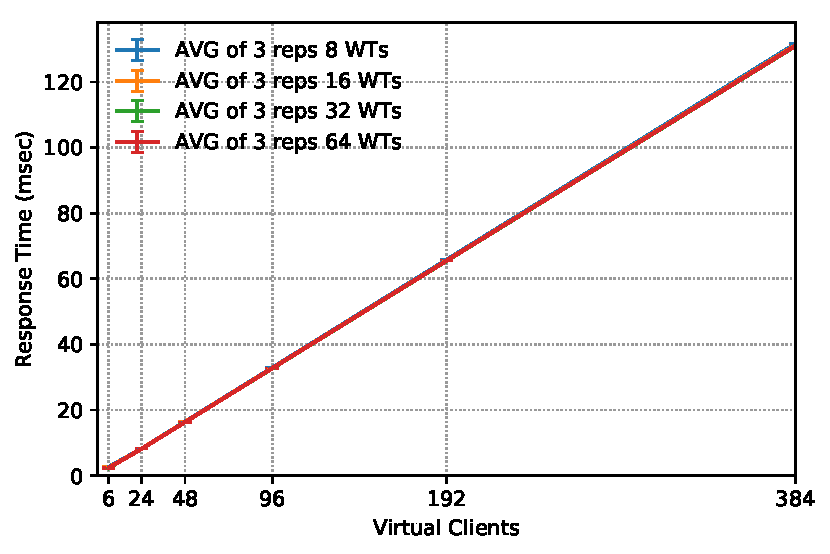
\includegraphics[width=0.6\textwidth]{figures/baseline_mw_1_mw/rt_memtier_read_only.pdf}
  }
\end{figure}

\begin{figure}[!h]
  \centering
    \caption{Plots for baseline with one Middleware (read-only MIDDLEWARE)}
  \label{fig:baseline_mw_1_mw_mw_ro}
  \makebox[\textwidth]{
    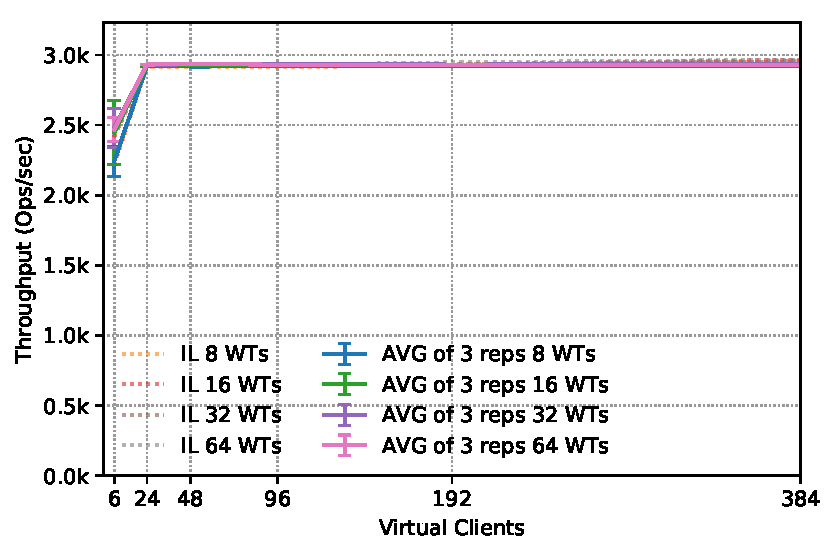
\includegraphics[width=0.6\textwidth]{figures/baseline_mw_1_mw/tp_middleware_read_only.pdf}
    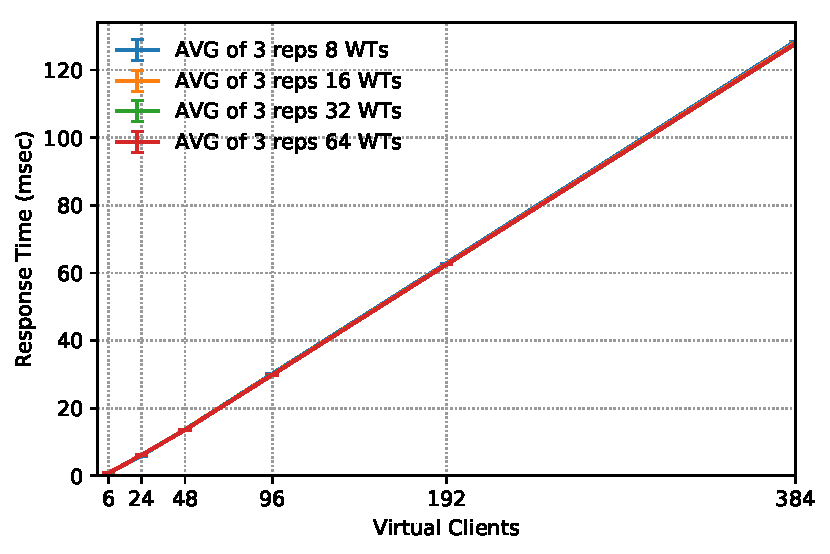
\includegraphics[width=0.6\textwidth]{figures/baseline_mw_1_mw/rt_middleware_read_only.pdf}
  }
\end{figure}

\begin{figure}[!h]
  \centering
    \caption{Plots for baseline with one Middleware, Service Time and Queue Waiting Time (read-only MIDDLEWARE)}
  \label{fig:baseline_mw_1_mw_mw_c_ro}
  \makebox[\textwidth]{
    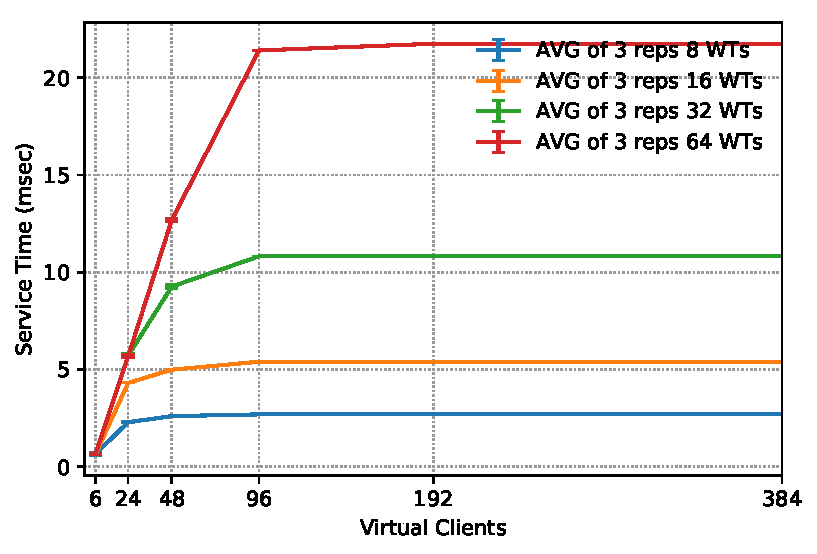
\includegraphics[width=0.6\textwidth]{figures/baseline_mw_1_mw/st_middleware_read_only.pdf}
    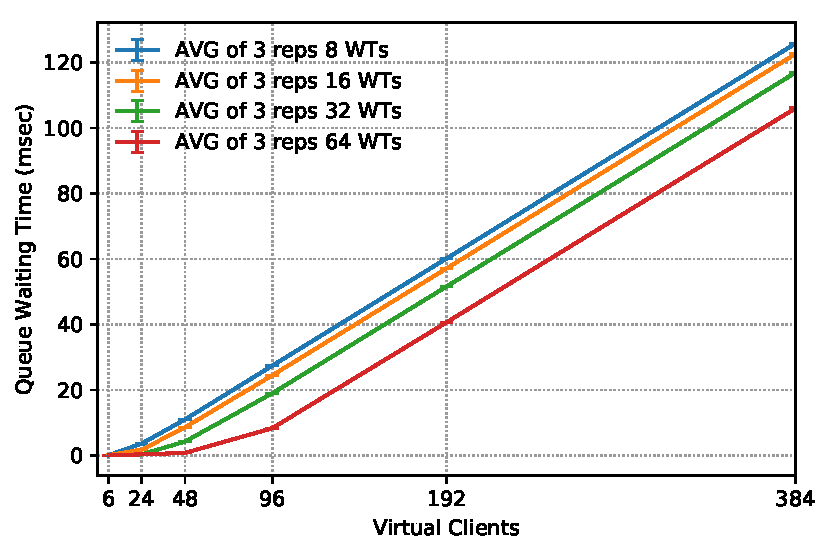
\includegraphics[width=0.6\textwidth]{figures/baseline_mw_1_mw/wt_middleware_read_only.pdf}
  }
\end{figure}

\begin{figure}[!h]
  \centering
    \caption{Plots for baseline with one Middleware (read-only MIDDLEWARE)}
  \label{fig:baseline_mw_1_mw_mw_ro}
  \makebox[\textwidth]{
    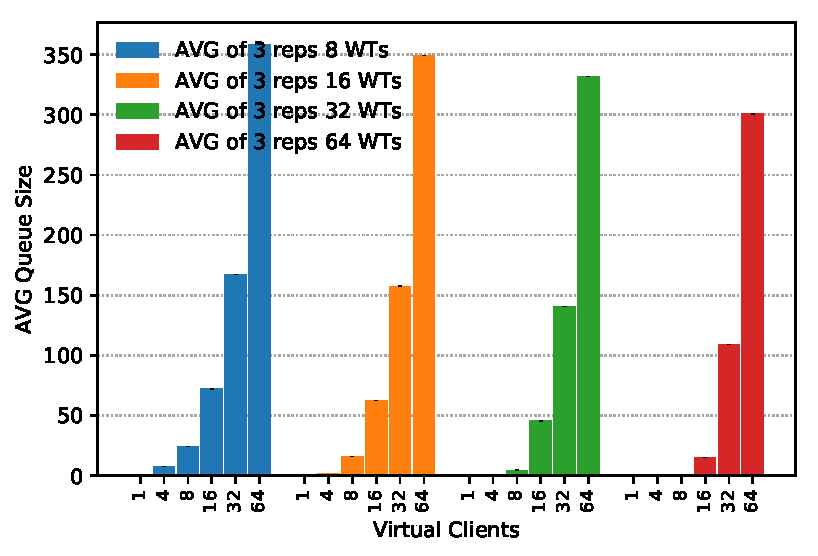
\includegraphics[width=0.6\textwidth]{figures/baseline_mw_1_mw/qs_middleware_read_only.pdf}
  }
\end{figure}

\subsubsection*{Write-Only}

As expected, increasing the number of worker threads in the middleware, results in an increase of the throughput. Even though, for every distinct worker thread configuration, we observe a distinct throughput behavior, there's a common treat that each configuration seems to manifest. In fact we can clearly identify and split the plot in two phases: one that goes from 6 to 192 \texttt{VCs}, and another one, that goes from 192 to 384 \texttt{VCs}. 
In the former (under-saturated phase), the configurations with 16, 32 and 64 workers, behave almost identically (apart from when we reach \texttt{VCs=96}, where we observe a difference of $\approx$ 500-600 $ops/s$).
The latter phase shows a much larger difference in performance for different worker threads configuration. We observe a clear distinction between 8 and 16 worker threads, and between 16 and 32, but not as much between 32 and 64 worker threads. 

\begin{figure}[!h]
  \centering
  \caption{Plots for baseline with one Middleware (write-only CLIENT)}
  \label{fig:baseline_mw_1_mw_mt_wo}
  \makebox[\textwidth]{
    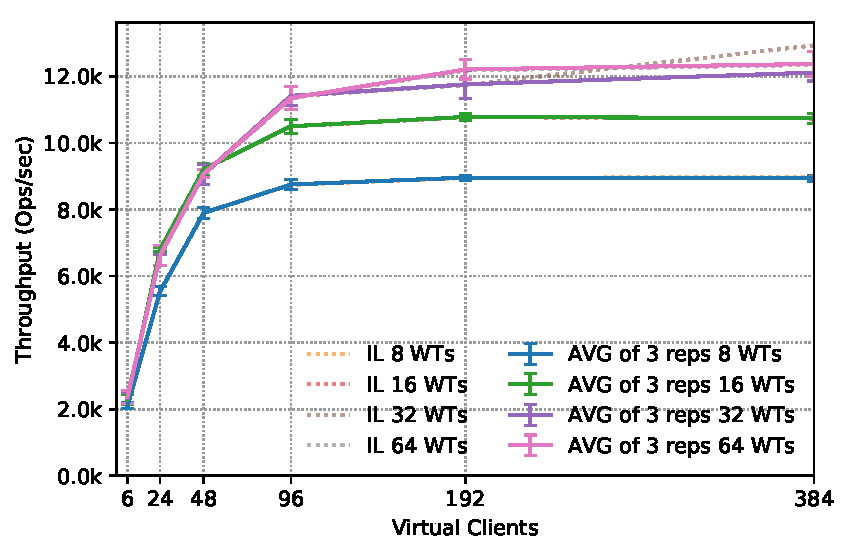
\includegraphics[width=0.6\textwidth]{figures/baseline_mw_1_mw/tp_memtier_write_only.pdf}
    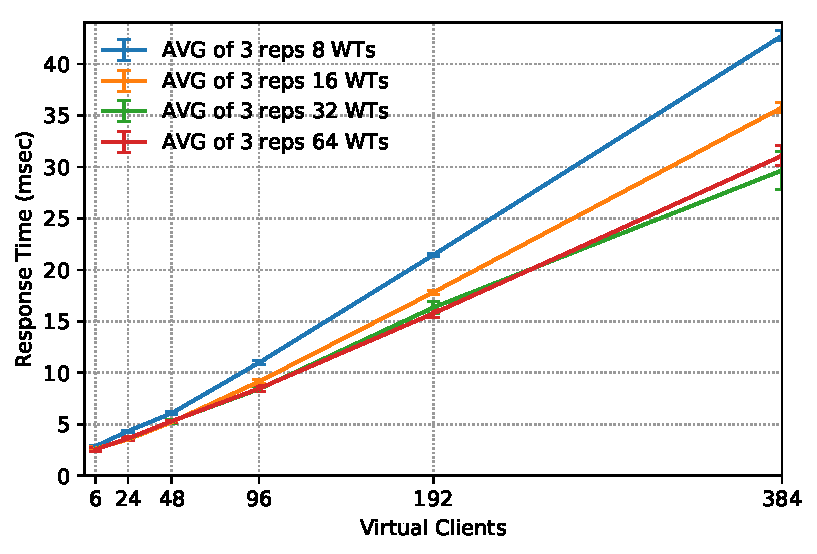
\includegraphics[width=0.6\textwidth]{figures/baseline_mw_1_mw/rt_memtier_write_only.pdf}
  }
\end{figure}

\begin{figure}[!h]
  \centering
  \caption{Plots for baseline with one Middleware (write-only MIDDLEWARE)}
  \label{fig:baseline_mw_1_mw_mw_wo}
  \makebox[\textwidth]{
    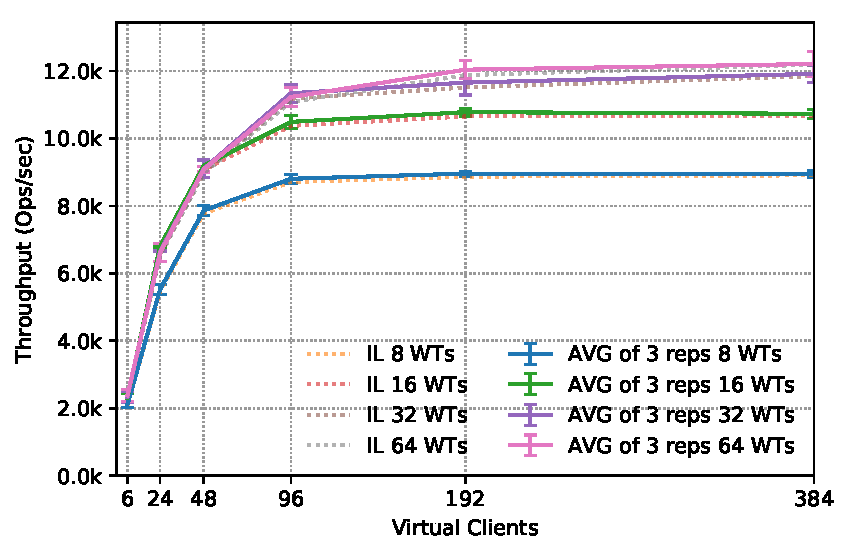
\includegraphics[width=0.6\textwidth]{figures/baseline_mw_1_mw/tp_middleware_write_only.pdf}
    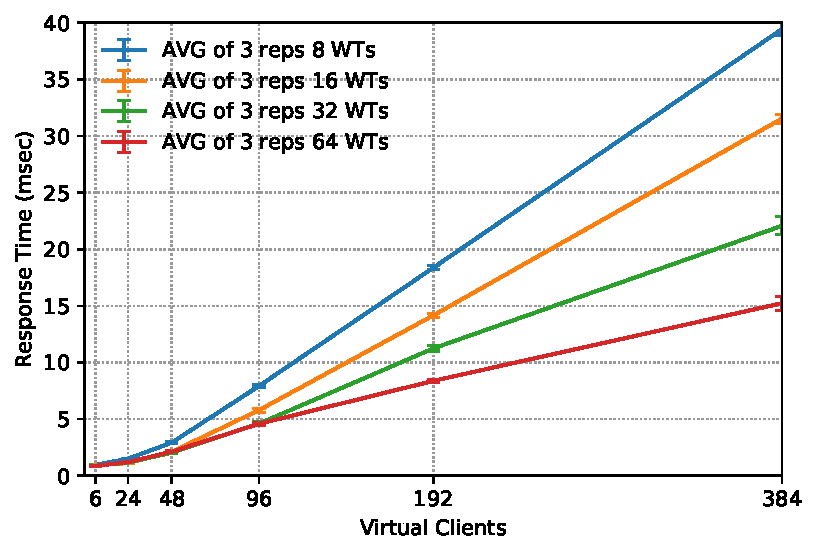
\includegraphics[width=0.6\textwidth]{figures/baseline_mw_1_mw/rt_middleware_write_only.pdf}
  }
\end{figure}

\begin{figure}[!h]
  \centering
  \caption{Plots for baseline with one Middleware, Service Time and Queue Waiting Time (write-only MIDDLEWARE)}
  \label{fig:baseline_mw_1_mw_mw_c_wo}
  \makebox[\textwidth]{
    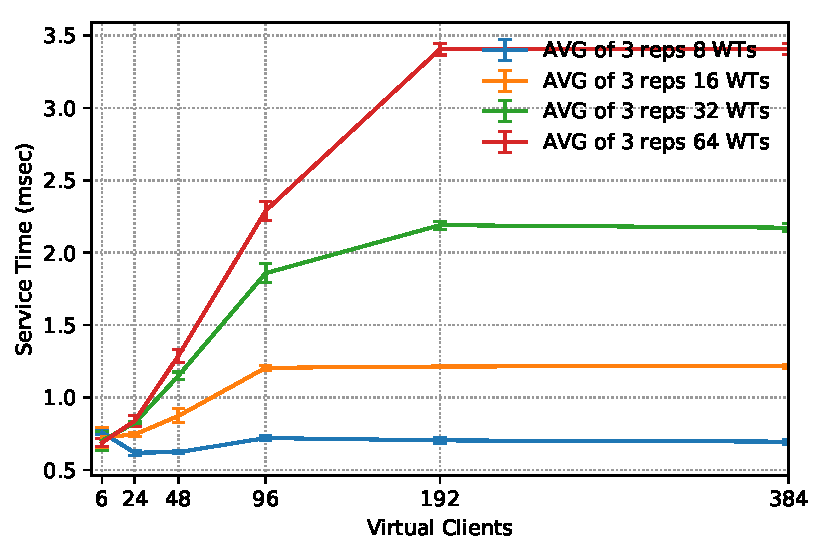
\includegraphics[width=0.6\textwidth]{figures/baseline_mw_1_mw/st_middleware_write_only.pdf}
    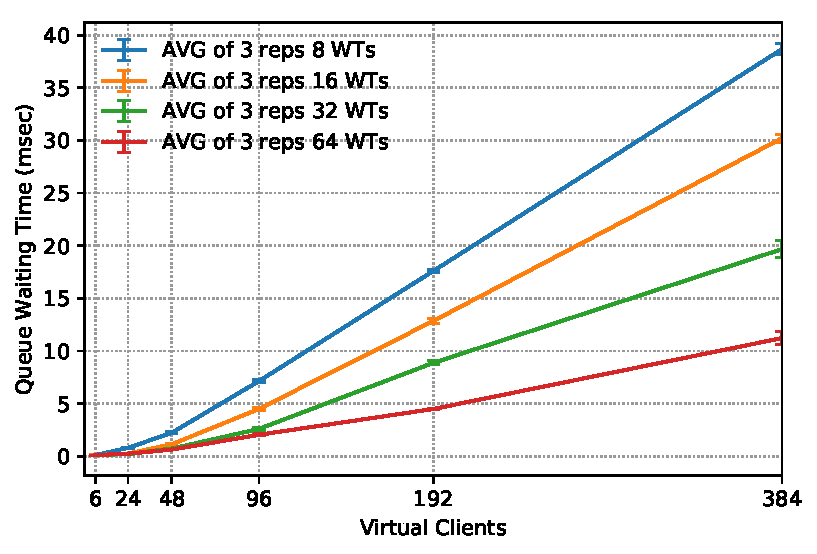
\includegraphics[width=0.6\textwidth]{figures/baseline_mw_1_mw/wt_middleware_write_only.pdf}
  }
\end{figure}

\begin{figure}[!h]
  \centering
    \caption{Plots for baseline with one Middleware, Average Queue Size (write-only MIDDLEWARE)}
  \label{fig:baseline_mw_1_mw_mw_qs_wo}
  \makebox[\textwidth]{
    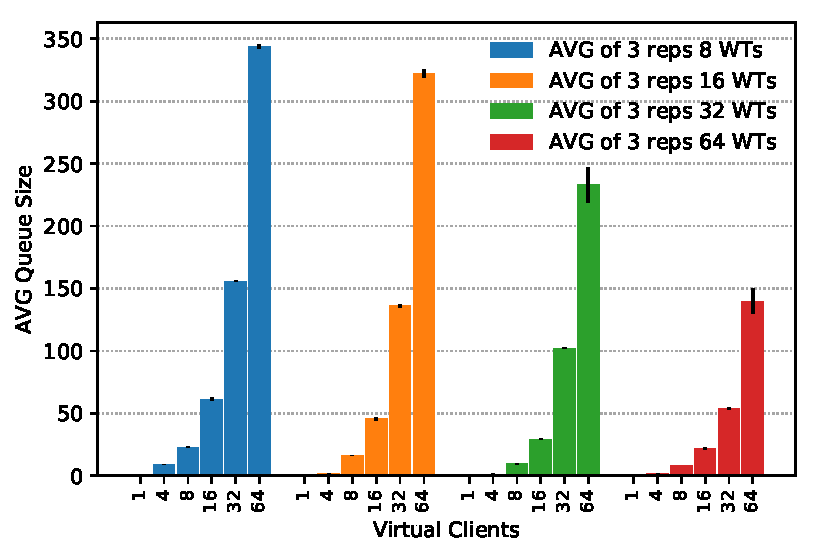
\includegraphics[width=0.6\textwidth]{figures/baseline_mw_1_mw/qs_middleware_write_only.pdf}
  }
\end{figure}

\subsection{Two Middlewares}

Connect three load generator machines (two instances of memtier with CT=1) to two middlewares and use 1 memcached server. Run a read-only and a write-only workload with increasing number of clients (between 2 and 64) and measure response time \emph{both at the client and at the middleware}, and plot the throughput and response time as measured in the middleware.

Repeat this experiment for different number of worker threads inside the middleware: 8, 16, 32, 64.

\begin{center}
	\scriptsize{
		\begin{tabular}{|l|c|}
			\hline Number of servers                & 1                        \\ 
			\hline Number of client machines        & 3                        \\ 
			\hline Instances of memtier per machine & 2                        \\ 
			\hline Threads per memtier instance     & 1                        \\
			\hline Virtual clients per thread       & [1..32]                  \\ 
			\hline Workload                         & Write-only and Read-only \\
			\hline Multi-Get behavior               & N/A                      \\
			\hline Multi-Get size                   & N/A                      \\
			\hline Number of middlewares            & 2                        \\
			\hline Worker threads per middleware    & [8..64]                  \\
			\hline Repetitions                      & 3 or more (at least 1 minute each)                \\ 
			\hline 
		\end{tabular}
	} 
\end{center}

\subsubsection{Explanation}

Provide a detailed analysis of the results (e.g., bottleneck analysis, component utilizations, average queue lengths, system saturation). Add any additional figures and experiments that help you illustrate your point and support your claims.

\subsection{Summary}

Based on the experiments above, fill out the following table. For both of them use the numbers from a single experiment to fill out all lines. Miss rate represents the percentage of GET requests that return no data. Time in the queue refers to the time spent in the queue between the net-thread and the worker threads.


\begin{center}
	{Maximum throughput for one middleware.}
	\begin{tabular}{|l|p{2cm}|p{2cm}|p{2cm}|p{2cm}|}
		\hline                                & Throughput & Response time & Average time in queue & Miss rate \\ 
		\hline Reads: Measured on middleware  &            &               &                       &           \\ 
		\hline Reads: Measured on clients     &            &               & n/a                   &           \\ 
		\hline Writes: Measured on middleware &            &               &                       & n/a       \\ 
		\hline Writes: Measured on clients    &            &               & n/a                   & n/a       \\ 
		\hline 
	\end{tabular}
\end{center}

\begin{center}
	{Maximum throughput for two middlewares.}
	\begin{tabular}{|l|p{2cm}|p{2cm}|p{2cm}|p{2cm}|}
		\hline                                & Throughput & Response time & Average time in queue & Miss rate \\ 
		\hline Reads: Measured on middleware  &            &               &                       &           \\ 
		\hline Reads: Measured on clients     &            &               & n/a                   &           \\ 
		\hline Writes: Measured on middleware &            &               &                       & n/a       \\ 
		\hline Writes: Measured on clients    &            &               & n/a                   & n/a       \\ 
		\hline 
	\end{tabular}
\end{center}

Based on the data provided in these tables, write at least two paragraphs summarizing your findings about the performance of the middleware in the baseline experiments.

\section{Throughput for Writes (90 pts)}

\subsection{Full System}

Connect three load generating VMs to two middlewares and three memchached servers. Run a write-only experiment. 
You need to plot throughput and response time measured on the middleware as a function of number of clients. The measurements have to be performed for 8, 16, 32 and 64 worker threads inside each middleware.

\begin{center}
	\scriptsize{
		\begin{tabular}{|l|c|}
			\hline Number of servers                & 3          \\ 
			\hline Number of client machines        & 3          \\ 
			\hline Instances of memtier per machine & 2          \\ 
			\hline Threads per memtier instance     & 1          \\
			\hline Virtual clients per thread       & [1..32]    \\ 
			\hline Workload                         & Write-only \\
			\hline Multi-Get behavior               & N/A        \\
			\hline Multi-Get size                   & N/A        \\
			\hline Number of middlewares            & 2          \\
			\hline Worker threads per middleware    & [8..64]    \\
			\hline Repetitions                      & 3 or more (at least 1 minute each)  \\ 
			\hline 
		\end{tabular}
	} 
\end{center}

\subsubsection{Explanation}

Provide a detailed analysis of the results (e.g., bottleneck analysis, component utilizations, average queue lengths, system saturation). Add any additional figures and experiments that help you illustrate your point and support your claims.

\subsection{Summary}

Based on the experiments above, fill out the following table with the data corresponding to the maximum throughput point for all four worker-thread scenarios.

\begin{center}
	{Maximum throughput for the full system}
	\begin{tabular}{|l|p{1.5cm}|p{1.5cm}|p{1.5cm}|p{1.5cm}|}
		\hline                                            & WT=8 & WT=16 & WT=32 & WT=64 \\ 
		\hline Throughput (Middleware)                    &      &       &       &       \\ 
		\hline Throughput (Derived from MW response time) &      &       &       &       \\ 
		\hline Throughput (Client)                        &      &       &       &       \\ 
		\hline Average time in queue                      &      &       &       &       \\ 
		\hline Average length of queue                    &      &       &       &       \\ 
		\hline Average time waiting for memcached         &      &       &       &       \\ 
		\hline 
	\end{tabular}
\end{center}

Based on the data provided in these tables, draw conclusions on the state of your system for a variable number of worker threads.

\section{Gets and Multi-gets (90 pts)}

For this set of experiments you will use three load generating machines, two middlewares and three memcached servers. Each memtier instance should have 2 virtual clients in total and the number of middleware worker threads is 64, or the one that provides the highest throughput in your system (whichever number of threads is smaller).

For multi-GET workloads, use the \texttt{--ratio} parameter to specify the exact ratio between SETs and GETs. You will have to measure response time on the client as a function of multi-get size, with and without sharding on the middlewares.

\subsection{Sharded Case}

Run multi-gets with 1, 3, 6 and 9 keys (memtier configuration) with sharding enabled (multi-gets are broken up into smaller multi-gets and spread across servers). Plot average response time as measured on the client, as well as the 25th, 50th, 75th, 90th and 99th percentiles.

\begin{center}
	\scriptsize{
		\begin{tabular}{|l|c|}
			\hline Number of servers                & 3                       \\ 
			\hline Number of client machines        & 3                       \\ 
			\hline Instances of memtier per machine & 2                       \\ 
			\hline Threads per memtier instance     & 1                       \\
			\hline Virtual clients per thread       & 2     		            \\ 
			\hline Workload                         & ratio=1:$<$Multi-Get size$>$             \\
			\hline Multi-Get behavior               & Sharded                 \\
			\hline Multi-Get size                   & [1..9]                  \\
			\hline Number of middlewares            & 2                       \\
			\hline Worker threads per middleware    & max. throughput config. \\
			\hline Repetitions                      & 3 or more (at least 1 minute each)               \\ 
			\hline 
		\end{tabular}
	} 
\end{center}

\subsubsection{Explanation}

Provide a detailed analysis of the results (e.g., bottleneck analysis, component utilizations, average queue lengths, system saturation). Add any additional figures and experiments that help you illustrate your point and support your claims.

\subsection{Non-sharded Case}

Run multi-gets with 1, 3, 6 and 9 keys (memtier configuration) with sharding disabled. Plot average response time as measured on the client, as well as the 25th, 50th, 75th, 90th and 99th percentiles.

\begin{center}
	\scriptsize{
		\begin{tabular}{|l|c|}
			\hline Number of servers                & 3                       \\ 
			\hline Number of client machines        & 3                       \\ 
			\hline Instances of memtier per machine & 2                       \\ 
			\hline Threads per memtier instance     & 1                       \\
			\hline Virtual clients per thread       & 2                		 \\ 
			\hline Workload                         & ratio=1:$<$Multi-Get size$>$              \\
			\hline Multi-Get behavior               & Non-Sharded             \\
			\hline Multi-Get size                   & [1..9]                  \\
			\hline Number of middlewares            & 2                       \\
			\hline Worker threads per middleware    & max. throughput config. \\
			\hline Repetitions                      & 3 or more (at least 1 minute each)               \\ 
			\hline 
		\end{tabular}
	} 
\end{center}

\subsubsection{Explanation}

Provide a detailed analysis of the results (e.g., bottleneck analysis, component utilizations, average queue lengths, system saturation). Add any additional figures and experiments that help you illustrate your point and support your claims.

\subsection{Histogram}

For the case with 6 keys inside the multi-get, display four histograms representing the sharded and non-sharded response time distribution, both as measured on the client, and inside the middleware. Choose the bucket size in the same way for all four, and such that there are at least 10 buckets on each of the graphs.

\subsection{Summary}

Provide a detailed comparison of the sharded and non-shareded modes. For which multi-GET size is sharding the preferred option? Provide a detailed analysis of your system. Add any additional figures and experiments that help you illustrate your point and support your claims.

\section{2K Analysis (90 pts)}

We perform a $2^kr$ experimental analysis to investigate the effect of ($k=3$) \textbf{factors}, namely:

\begin{itemize}
    \item The number of memcached servers
    \item The number of middlewares
    \item The number of worker threads per middleware
\end{itemize}

and study the effects of each of them on throughput and response time respectively (\textbf{response variables}).

\subsection{Experiment setting}

There are 3 machines that generate workloads. Then based on the number of middlewares (1 or 2), each client machine runs (1 or 2) instances of memtier, each with 32 virtual clients and (2 or 1) threads respectively. In the case of two memtier instances per machine, each of them connects to a different middleware. 
Each middleware runs either (8 or 32) worker threads, and is connected to either (2 or 3) mecached machines. We measure both throughput and response time for each workload (read-only and write-only).
We investigate experimental errors by replicating each experiment 3 times ($r=3$), so the response variable, is simply the average between each repetition.
Based on results on experiments in section~\ref{sec:3.1}, we do expect the number of middlewares and the number of worker threads, to have relevant impact on the response variables. Furthermore, we do assume that the effects of the factor are additive and that measurements error are independent and follow a normal distribution.\\

\begin{center}
	\scriptsize{
		\begin{tabular}{|l|c|}
			\hline Number of servers                & 1 and 3                                     \\ 
			\hline Number of client machines        & 3                                           \\ 
			\hline Instances of memtier per machine & 1 (1 middleware) or 2 (2 middlewares) \\ 
			\hline Threads per memtier instance     & 2 (1 middleware) or 1 (2 middlewares)   \\
			\hline Virtual clients per thread       &  32                                     \\ 
			\hline Workload                         & Write-only and Read-only\\
			\hline Multi-Get behavior               & N/A                                         \\
			\hline Multi-Get size                   & N/A                                         \\
			\hline Number of middlewares            & 1 and 2                                     \\
			\hline Worker threads per middleware    & 8 and 32                                    \\
			\hline Repetitions                      & 3 or more (at least 1 minute each)                                   \\ 
			\hline 
		\end{tabular}
	} 
\end{center}

\subsection{Model}

We model the response variable $y$ as\\
\begin{equation}
    y = q_0 + q_Ax_A + q_Bx_B + q_Cx_C + q_{AB}x_Aa_B + q_{AC}x_Ax_C + q_{BC}x_Bx_C + q_{ABC}x_Ax_Bx_C + \epsilon
\end{equation}

where $x_A, x_B, x_C$ are defined as\\
\begin{align*}
x_A &= 
\begin{cases}
    -1 & \text{ if 1 server}\\
    1 & \text{ if 3 servers}
\end{cases}
\\
x_B &=
\begin{cases}
    -1 & \text{ if 1 middleware}\\
    1 & \text{ if 2 middlewares}
\end{cases}
\\
x_C &=
\begin{cases}
    -1 & \text{ if 8 worker threads}\\
    1 & \text{ if 32 worker threads}
\end{cases}
\end{align*}

and $q_0, q_A, \dots q_{ABC},$ and $\epsilon$ (\textbf{experimental error}) are the parameters to be computed with the \textit{Sign Table Method}.

\subsection{Results}

\subsubsection{Throughput}

\paragraph{Read-Only}

\begin{tabu}{|r|r|r|r|r|r|r|r|r|r|r|r|r|}
\hline
    \rowfont[c]{\bfseries} i & I & A & B & C & AB & AC & BC & ABC & $y_1$ & $y_2$ & $y_3$ & $\hat{y}$\\ \hline
    1 & 1 & -1 & -1 & -1 & 1 & 1 & 1 & -1 & 0.0 & 0.0 & 0.0 & 0.0\\ \hline
    2 & 1 & -1 & -1 & 1 & 1 & -1 & -1 & 1 & 0.0 & 0.0 & 0.0 & 0.0\\ \hline
    3 & 1 & -1 & 1 & -1 & -1 & 1 & -1 & 1 & 0.0 & 0.0 & 0.0 & 0.0\\ \hline
    4 & 1 & -1 & 1 & 1 & -1 & -1 & 1 & -1 & 0.0 & 0.0 & 0.0 & 0.0\\ \hline
    5 & 1 & 1 & -1 & -1 & -1 & -1 & 1 & 1 & 0.0 & 0.0 & 0.0 & 0.0\\ \hline
    6 & 1 & 1 & -1 & 1 & -1 & 1 & -1 & -1 & 0.0 & 0.0 & 0.0 & 0.0\\ \hline
    7 & 1 & 1 & 1 & -1 & 1 & -1 & -1 & -1 & 0.0 & 0.0 & 0.0 & 0.0\\ \hline
    8 & 1 & 1 & 1 & 1 & 1 & 1 & 1 & 1 & 0.0 & 0.0 & 0.0 & 0.0\\ \hline
\end{tabu}

\paragraph{Write-Only}

\begin{tabu}{|r|r|r|r|r|r|r|r|r|r|r|r|r|}
\hline
    \rowfont[c]{\bfseries} i & I & A & B & C & AB & AC & BC & ABC & $y_1$ & $y_2$ & $y_3$ & $\hat{y}$\\ \hline
    1 & 1 & -1 & -1 & -1 & 1 & 1 & 1 & -1 & 0.0 & 0.0 & 0.0 & 0.0\\ \hline
    2 & 1 & -1 & -1 & 1 & 1 & -1 & -1 & 1 & 0.0 & 0.0 & 0.0 & 0.0\\ \hline
    3 & 1 & -1 & 1 & -1 & -1 & 1 & -1 & 1 & 0.0 & 0.0 & 0.0 & 0.0\\ \hline
    4 & 1 & -1 & 1 & 1 & -1 & -1 & 1 & -1 & 0.0 & 0.0 & 0.0 & 0.0\\ \hline
    5 & 1 & 1 & -1 & -1 & -1 & -1 & 1 & 1 & 0.0 & 0.0 & 0.0 & 0.0\\ \hline
    6 & 1 & 1 & -1 & 1 & -1 & 1 & -1 & -1 & 0.0 & 0.0 & 0.0 & 0.0\\ \hline
    7 & 1 & 1 & 1 & -1 & 1 & -1 & -1 & -1 & 0.0 & 0.0 & 0.0 & 0.0\\ \hline
    8 & 1 & 1 & 1 & 1 & 1 & 1 & 1 & 1 & 0.0 & 0.0 & 0.0 & 0.0\\ \hline
\end{tabu}

\subsubsection{ResponseTime}

\paragraph{Read-Only}

\begin{tabu}{|r|r|r|r|r|r|r|r|r|r|r|r|r|}
\hline
    \rowfont[c]{\bfseries} i & I & A & B & C & AB & AC & BC & ABC & $y_1$ & $y_2$ & $y_3$ & $\hat{y}$\\ \hline
    1 & 1 & -1 & -1 & -1 & 1 & 1 & 1 & -1 & 0.0 & 0.0 & 0.0 & 0.0\\ \hline
    2 & 1 & -1 & -1 & 1 & 1 & -1 & -1 & 1 & 0.0 & 0.0 & 0.0 & 0.0\\ \hline
    3 & 1 & -1 & 1 & -1 & -1 & 1 & -1 & 1 & 0.0 & 0.0 & 0.0 & 0.0\\ \hline
    4 & 1 & -1 & 1 & 1 & -1 & -1 & 1 & -1 & 0.0 & 0.0 & 0.0 & 0.0\\ \hline
    5 & 1 & 1 & -1 & -1 & -1 & -1 & 1 & 1 & 0.0 & 0.0 & 0.0 & 0.0\\ \hline
    6 & 1 & 1 & -1 & 1 & -1 & 1 & -1 & -1 & 0.0 & 0.0 & 0.0 & 0.0\\ \hline
    7 & 1 & 1 & 1 & -1 & 1 & -1 & -1 & -1 & 0.0 & 0.0 & 0.0 & 0.0\\ \hline
    8 & 1 & 1 & 1 & 1 & 1 & 1 & 1 & 1 & 0.0 & 0.0 & 0.0 & 0.0\\ \hline
\end{tabu}

\paragraph{Write-Only}

\begin{tabu}{|r|r|r|r|r|r|r|r|r|r|r|r|r|}
\hline
    \rowfont[c]{\bfseries} i & I & A & B & C & AB & AC & BC & ABC & $y_1$ & $y_2$ & $y_3$ & $\hat{y}$\\ \hline
    1 & 1 & -1 & -1 & -1 & 1 & 1 & 1 & -1 & 0.0 & 0.0 & 0.0 & 0.0\\ \hline
    2 & 1 & -1 & -1 & 1 & 1 & -1 & -1 & 1 & 0.0 & 0.0 & 0.0 & 0.0\\ \hline
    3 & 1 & -1 & 1 & -1 & -1 & 1 & -1 & 1 & 0.0 & 0.0 & 0.0 & 0.0\\ \hline
    4 & 1 & -1 & 1 & 1 & -1 & -1 & 1 & -1 & 0.0 & 0.0 & 0.0 & 0.0\\ \hline
    5 & 1 & 1 & -1 & -1 & -1 & -1 & 1 & 1 & 0.0 & 0.0 & 0.0 & 0.0\\ \hline
    6 & 1 & 1 & -1 & 1 & -1 & 1 & -1 & -1 & 0.0 & 0.0 & 0.0 & 0.0\\ \hline
    7 & 1 & 1 & 1 & -1 & 1 & -1 & -1 & -1 & 0.0 & 0.0 & 0.0 & 0.0\\ \hline
    8 & 1 & 1 & 1 & 1 & 1 & 1 & 1 & 1 & 0.0 & 0.0 & 0.0 & 0.0\\ \hline
\end{tabu}

\section{Queuing Model (90 pts)}

Note that for queuing models it is enough to use the experimental results from the previous sections. It is, however, possible that the numbers you need are not only the ones in the figures we asked for, but also the internal measurements that you have obtained through instrumentation of your middleware.

\subsection{M/M/1}

Build queuing model based on Section 4 (write-only throughput) for each worker-thread configuration of the middleware. Use one M/M/1 queue to model your entire system. Motivate your choice of input parameters to the model. Explain for which experiments the predictions of the model match and for which they do not.

\subsection{M/M/m}

Build an M/M/m model based on Section 4, where each middleware worker thread is represented as one service.  Motivate your choice of input parameters to the model. Explain for which experiments the predictions of the model match and for which they do not.

\subsection{Network of Queues}

Based on Section 3, build a network of queues which simulates your system. Motivate the design of your network of queues and relate it wherever possible to a component of your system. Motivate your choice of input parameters for the different queues inside the network. Perform a detailed analysis of the utilization of each component and clearly state what the bottleneck of your system is. Explain for which experiments the predictions of the model match and for which they do not.

\end{document}
